% !TeX spellcheck = en_US

\section{Advanced topics}\label{MoreExamples}

\subsection{Computations with a polytope}\label{Polytopes}

In many cases the starting point of a computation is a polytope, i.e., a bounded polyhedron -- and not a cone or monoid. Normaliz offers two types of input for polytopes that allow almost the same computations, namely
\begin{arab}
	\item \emph{homogeneous} input type for which the polytope is the intersection of a cone with a hyperplane defined by the grading (automatically bounded): $P=\{x\in C:\deg x=1\}$.
	\item \emph{inhomogeneous} input defining a polytope (and not an unbounded polyhedron).
\end{arab}
A problem that can arise with homogeneous input is the appearance of a grading enumerator $g>1$. In this case the polytope $P$ defined by the input grading is replaced by $gP$. This may be undesirable and can therefore be blocked by \verb|NoGradingDenom|. Note: a grading denominator $g>1$ can only appear if the affine space spanned by the polytope does not contain a lattice point. This is a rare situation, but nevertheless you may want to safeguard against it.

Computation goals whose names have a ``polytopal touch'' (as opposed to ``algebraic touch'') set \verb|NoGradingDenom| automatically. These computation goals are also to be used with inhomogeneous input; see the following table. The homogeneous input type \verb|polytope| sets \verb|NoGradingDenom| as well.

In the following table $L$ is the lattice of reference defined by the input data.

\begin{center}
	\begin{tabular}[pos]{|c|c|c|}
		\hline
		& inhom input or& hom input\\
		desired data & hom input blocking & allowing\\
		&grading denominator& grading denominator\\
		\hline\hline
		lattice points &\verb|LatticePoints|&\verb|Deg1Elements|\\
		\hline
		number of lattice points& \verb|NumberLatticePoints|& ---\\
		\hline
		convex hull of&&\\
		lattice points& \verb|IntegerHull|& ---\\
		\hline
		generating function of&&\\
		$k\mapsto \#(kP\cap L) $&\verb|EhrhartSeries|&\verb|HilbertSeries|\\
		\hline
		volume or&&\\
		multiplicity& \verb|Volume|&\verb|Multiplicity|\\
		\hline
		integral&\verb|Integral|&---\\
		\hline
	\end{tabular}
\end{center}

Note that \verb|HilbertSeries| and \verb|Multiplicity| make also sense with inhomogeneous input, but they refer to a different counting function, namely
$$
k\mapsto \#(x\in P\cap L, \deg x=k).
$$
Even if $P$ is a polytope, this function has applications; see Section~\ref{count}. Note that inhomogeneous input sets \verb|NoGradingDenom|.

\subsubsection{Lattice normalized and Euclidean volume}\label{volume}

As just mentioned, for polytopes defined by homogeneous input Normaliz has two computation goals, \verb|Multiplicity|, \verb|-v|, and \verb|Volume, -V|, that are almost identical: \verb|Volume| = \verb|Multiplicity| + \verb|NoGradingDenom|. Both compute the lattice normalized volume; moreover, \verb|Volume | additionally computes the Euclidean volume and can also be used with inhomogeneous input, for which \verb|Multiplicity| has a different meaning. (For the algebraic origin of \verb|Multiplicity| see Appendix~\ref{AppHilbertSeries}.)

In the following we want to clarify the notion of \emph{lattice normalized volume}.

(1) Let $P\subset\RR^d$ be a polytope of dimension $r$ and let $A$ be the affine subspace spanned by $P$. Then the Euclidean volume $\vol_{\textup{eucl}}(P)$ of $P$ is computed with respect to the $r$-dimensional Lebesgue measure in which an $r$-dimensional cube in $A$ of edge length $1$ has measure $1$.

(2) For the lattice normalized volume we need a lattice $L$ of reference. We assume that $\aff(P)\subset\aff(L)$. (It would be enough to have this inclusion after a parallel translation of $\aff(P)$.) Choosing the origin in $L$, one can assume that $\aff(L)$ is a vector subspace of $\RR^d$ so that we can identify it with $\RR^d$ after changing $d$ if necessary. After a coordinate transformation we can further assume that $L=\ZZ^d$ (in general this is not an orthogonal change of coordinates!). To continue we need that $\aff(P)$ is a rational subspace. There exists $k\in\NN$ such that $k\aff(P)$ contains a lattice simplex. The lattice normalized volume $\vol_L$ of $kP$ is then given by the Lebesgue measure on $k\aff(P)$ in which the smallest possible lattice simplex in $k\aff(P)$ has volume $1$. Finally we set $\vol_L(P)=\vol_L(kP)/k^r$ where $r=\dim(P)$.

If $P$ is a full-dimensional polytope in $\RR^d$ and $L=\ZZ^d$, then $\vol_L(P)=d!\vol_{\textup{eucl}}(P)$, but in general the correction factor is $cr!$ with $c$ depending on $\aff(P)$: the line segment in $\RR^2$ connecting $(1,0)$ and $(0,1)$ has euclidean length $\sqrt{2}$, but lattice normalized volume $1$. As this simple example shows, $c$ can be irrational.

\subsubsection{Developer's choice: homogeneous input}

Our recommendation: if you have the choice between homogeneous and inhomogeneous input, go homogeneous (with \verb|NoGradingDenom| if necessary). You do not lose any computation goal and can only gain efficiency.

\subsection{Lattice points in polytopes once more}\label{LattPoints}

Normaliz has three main algorithms for the computation of lattice points of which two have two variants each:
\begin{arab}
	\item the project-and-lift algorithm (\verb|Projection, -j|),
	\item its variant using floating point arithmetic (\verb|ProjectionFloat, -J|),
	\item the triangulation based Normaliz primal algorithm specialized to lattice points\\ (\verb|PrimalMode, -P|),
	\item its variant using approximation of rational polytopes (\verb|Approximate, -r|),
	\item the dual algorithm specialized to lattice points (\verb|DualMode, -d|).
\end{arab}

The options \verb|Projection|, \verb|ProjectionFloat| and \verb|Approximate| do not imply a computation goal. Since \verb|PrimalMode| can also be used for the computation of Hilbert series and Hilbert bases, one must add the computation goal to it. In the homogeneous case one must add the computation goal also to \verb|DualMode|.

\emph{Remark.}\enspace
The triangulation based primal algorithm and the dual algorithm do not depend on the embedding of the computed objects into the ambient space since they use only data that are invariant under coordinate transformations. This is not true for project-and-lift and the approximation discussed below. Often \verb|Projection| and \verb|ProjectionFloat| (and in certain cases also \verb|PrimalMode|) profit significantly from LLL reduced coordinates (since version~3.4.1). We discuss this feature in Section~\ref{LLL}.

We recommend the reader to experiment with the following input files:
\begin{itemize}
	\item \verb|5x5.in|
	\item \verb|6x6.in|
	\item \verb|max_polytope_cand.in|
	\item \verb|hickerson-18.in|
	\item \verb|knapsack_11_60.in|
	\item \verb|ChF_2_64.in|
	\item \verb|ChF_8_1024.in|
	\item \verb|VdM_16_1048576.in| (may take some time)
	\item \verb|pedro2.in|
	\item \verb|pet.in|
	\item \verb|baby.in|
\end{itemize}

In certain cases you must use \verb|-i| on the command line to override the options in the input file if you want to try other options.

\verb|max_polytope_cand.in| came up in connection with the paper ``Quantum jumps of normal polytopes'' by W.~Bruns, J.~Gubeladze and M.~Micha\l{}ek, Discrete Comput.\ Geom.\ 56 (2016), no.\ 1, 181--215. \verb|hickerson-18.in| is taken from the LattE distribution~\cite{LatInt}. \verb|pedro2.in| was suggested by P.~Garcia-Sanchez.

The files \verb|ChF*.in| and \verb|VdM*.in| are taken from the paper ``On the orthogonality of the Chebyshev-Frolov lattice and applications'' by Ch.~Kacwin, J.~Oettershagen and T.~Ullrich (Monatsh.\ Math.\ 184 (2017), 425--441). The file \verb|VdM_16_1048576.in| is based on the linear map given directly by the Vandermonde matrix. A major point of the paper is a coordinate transformation that simplifies computations significantly, and the files \verb|ChF*.in| are based on it.

The files \verb|pet.in| and \verb|baby.in| have been created in connection with the work on fusion rings. See \cite{ABPP}.

\subsubsection{Project-and-lift}\label{project}

We have explained the project-and-lift algorithm in Section~\ref{project_example}.
This algorithm is very robust arithmetically since it needs not compute determinants or solve systems of linear equations. Moreover, the project-and-lift algorithm itself does not use the vertices of the polytope explicitly and only computes lattice points in $P$ and its successive projections. Therefore it is rather insensitive against rational vertices with large denominators. (To get started it must usually compute the vertices of the input polytope; an exception are parallelotopes, as mentioned in Section~\ref{project_example} and discussed below.) Project-and-lift is not done by default if the number of support hyperplanes exceeds that of the number of extreme rays by a factor $>100$.

The option for project-and-lift is
\begin{itemize}
	\itemtt [Projection, -j]
\end{itemize}

There are two complications that may slow it down unexpectedly: (i) the projections may have large numbers of support hyperplanes, as seen in the example \verb|VdM_16_1048576.in| (it uses floating point arithmetic in the lifting part):
\begin{Verbatim}
Projection
embdim 17 inequalities 32
embdim 16 inequalities 240
...
embdim 11 inequalities 22880
embdim 10 inequalities 25740
embdim 9 inequalities 22880
...
embdim 3 inequalities 32
embdim 2 inequalities 2
\end{Verbatim}

(ii) The projections may have many lattice points that cannot be lifted to the top. As an example we look at the terminal output of \verb|pedro2.in|:
\begin{Verbatim}
embdim 2 LatticePoints 40
embdim 3 LatticePoints 575
embdim 4 LatticePoints 6698
embdim 5 LatticePoints 6698
embdim 6 LatticePoints 2
\end{Verbatim}

Despite of these potential problems, \verb|Projection| is the default choice of Normaliz for the computation of lattice points (if not combined with Hilbert series or Hilbert basis). If you do not want to use it, you must either choose another method explicitly or switch it off by \verb|NoProjection|. Especially for lattice polytopes with few extreme rays, but many support hyperplanes the triangulation base algorithm is often the better choice.

\emph{Parallelotopes.}\enspace
Lattice points in parallelotopes that are defined by inequalities, like those in the input files \verb|VdM*.in|, can be computed without any knowledge of the vertices. In fact, for them it is favorable to present a face $F$ by the list of facets whose intersection $F$ is (and not by the list of the $2^{\dim F}$ vertices of $F$!). Parallelotopes are not only simple polytopes. It is important that two faces do not intersect if and only if they are contained in parallel facets, and this is easy to control. Normaliz recognizes parallelotopes by itself, and suppresses the computation of the vertices unless asked to compute them.

\subsubsection{Project-and-lift with floating point arithmetic}

Especially the input of floating point numbers often forces Normaliz into GMP arithmetic. Since GMP arithmetic is slow (compared to arithmetic with machine integers or floating point numbers), Normaliz has a floating point variant of the project-and-lift algorithm. (Such an algorithm makes no sense for Hilbert bases or Hilbert series.) It behaves very well, even in computations for lower dimensional polytopes. We have not found a single deviation from the results with GMP arithmetic in our examples. Nevertheless, the projection phase is done in the in integer arithmetic, and only the lifting uses floating point.

The option for the floating point variant of project-and-lift is
\begin{itemize}
	\itemtt [ProjectionFloat, -J]
\end{itemize}
If you want a clear demonstration of the difference between \verb|Projection| and \verb|ProjectionFloat|, try \verb|VdM_16_1048576.in|.

The use of \verb|ProjectionFloat| or any other algorithmic variant is independent of the input type. The coordinates of the lattice points computed by \verb|ProjectionFloat| are assumed to be at most~$64$~bits wide, independently of the surrounding integer type. If this condition should not be satisfied in your application, you must use \verb|Projection| instead.

\subsubsection{LLL reduced coordinates and relaxation}\label{LLL}

The project-and-lift algorithm depends very much on the embedding of the polytope in the ambient space. We use LLL reduction to find coordinate transformations of the ambient space in which the vertices of the polytope have small coordinates so that the successive projections have few lattice points. Roughly speaking, LLL reduced coordinates are computed as follows. We form a matrix $A$ whose \emph{rows} are the vertices or the support hyperplanes of the polytope, depending on the situation. Suppose $A$ has $d$ columns; $A$ need not have integral entries, but it must have rank $d$. Then we apply LLL reduction to the lattice generated by the \emph{columns} of $A$. This amounts to finding a matrix $U\in \operatorname{GL}(d,\ZZ)$ such that the columns of $AU$ are short vectors (in the Euclidean norm). The matrix $U$ and its inverse then define the coordinate transformations forth and back.

Often LLL reduction has a stunning effect. We have a look at the terminal output of \verb|pedro2.in| run with \verb|-P|. The left column shows the present version, the right one is produced by Normaliz~3.4.0:
\begin{Verbatim}
embdim 2 LatticePoints 2              embdim 2 LatticePoints 40
embdim 3 LatticePoints 2              embdim 3 LatticePoints 672
embdim 4 LatticePoints 2              embdim 4 LatticePoints 6698
embdim 5 LatticePoints 3              embdim 5 LatticePoints 82616047
embdim 6 LatticePoints 2              embdim 6 LatticePoints 2
\end{Verbatim}

We have no example for which LLL increases the computation time. Though its application not seem to be a real disadvantage, it can be switched off for \verb|Projection| and \verb|ProjectionFloat| by
\begin{itemize}
	\itemtt[NoLLL]
\end{itemize}
Without LLL certain computations are simply impossible -- just try \verb|VdM_16_1048576| with \verb|NoLLL|. (This option is used internally to avoid a repetition of LLL computations.)

We use the original LLL original algorithm with the factor $0.9$.

Another aspect of the implementation that must be mentioned is the relaxation of inequalities: for the intermediate lifting of lattice points Normaliz uses at most $1000$ (carefully chosen) inequalities. Some additional intermediate lattice points are acceptable if the evaluation of inequalities is reduced by a substantial factor. On the left we see \verb|VdM_16_1048576| with relaxation, on the right without:
\begin{Verbatim}
...                                       ...
embdim 6 LatticePoints 2653                embdim 6 LatticePoints 2297
...                                       ...
embdim 10 LatticePoints 431039             embdim 10 LatticePoints 128385
embdim 11 LatticePoints 1031859            embdim 11 LatticePoints 277859
embdim 12 LatticePoints 2016708            embdim 12 LatticePoints 511507
embdim 13 LatticePoints 2307669            embdim 13 LatticePoints 806301
...                                       ...
\end{Verbatim}
No surprise that relaxation increases the number of intermediate lattice points, but it reduces the computation time by about a factor $2$.

It is of course not impossible that relaxation exhausts RAM or extends the computation time. Therefore one can switch it off by
\begin{itemize}
	\itemtt[NoRelax]
\end{itemize}

\subsubsection{Positive systems, coarse project-and-lift and patching}\label{positive_systems}

We call a system of linear equations and inequalities \emph{positive} if the inequalities contain the sign inequalities $x_i \ge 0$ for all coordinates and inequalities (including inequalities implied by equations) for all $i$ of type
\begin{equation}
\xi_1x_1 + \dots + \xi_{i-1}x_{i-1} + \xi_i x_i +  \xi_{i+1}x_{i+1} +\dots +  \xi_{d}x_{d} \le \eta \label{upper_bound}
\end{equation}
where $\xi_j \ge 0$ for all $j$ and $\xi_i >0$. This allows one to find an a priori upper bound for every coordinate $x_i$. For homogeneous input this must be modified a little: the grading must be a coordinate function, this coordinate is omitted on the left hand side, and $\eta$ is the coefficient of the coordinate that represents the grading.

For positive systems it is a priori clear that the polyhedron defined by the linear constraints is a polytope, and there is no need to check that by computing the vertices. Moreover, we can base a relaxed version of project-and-lift on the nonnegativity inequalities and the upper bounds \ref{upper_bound}.  This variant often has a tremendous advantage: run \verb|pet.in| as it is or with the option
\begin{itemize}
	\itemtt[NoCoarseProjection]
\end{itemize}
The computation times are $< 1$ sec and (most likely) $\sim\infty$.

Under certain conditions coarse project-and-lift is modified. Instead of proceeding from one coordinate to the next, ``local systems'' are used to extend the range of coordinates by ``patching''. It is a particularly fast method if it applies. Our standard example \verb|pet.in| is automatically run in this mode, unless you forbid it by
\begin{itemize}
	\itemtt[NoPatching]
\end{itemize}
To see the effect, try \verb|baby.in| as it is and with \verb|NoPatching|.

The patching algorithm and the use of polynomial equations was developed for computations of fusion rings reported in \cite{ABPP} and extensions.

It is possible  to save memory by using the option
\begin{itemize}
	\itemtt[ShortInt]
\end{itemize}
It saves the ``local solutions'' as 16 bit integers. The range is of course checked, and if it iss exceeded, Normaliz throws a \verb*|NoComputationException|.

Note that the patching algorithm allows distributed computation (se Section \ref{DistPatch}).

\subsubsection{Polynomial constraints for lattice points}\label{poly_const}

The lattice points in polytopes computed by Normaliz can be further constrained by polynomial equations an d inequalities (see Section \ref{poly_const_input}). For all algorithms different from project-and-lift the lattice points must be computed completely before the polynomial constraints can be used. It is a significant advantage of project-and-lift and its variants that every polynomial constraint can be applied as soon as all coordinates appearing  in it with a nonzero coefficient have been collected. This helps enormously to stop the extension of coordinates. 

To avoid ambiguities, only computation goals for lattice points in polytopes and convex hull data can be computed in the presence of polynomial constraints. 

\verb|pet.in|, \verb|baby.in| and \verb*|poly_equ.in| are examples with polynomial constraints.

\subsubsection{The patching order}\label{patch_order}

If polynmomial equations are present, then Normaliz tries to use them with as few coordinates as possible and schedules the patching algorithm accordingly. However, this can have a negative effect if it makes ``bad'' patches being used too early. Also congruences, whether explicitly given in the input or derived by Normaliz from linear equations, can influence the insertion order of the patches. 

There are some options that can modify the default behavior:
\begin{itemize}
	\itemtt[UseWeightsPatching, -{}-UWP] gives a ``weight'' to the coordinates so that ```bad'' patches are biased negatively.
	
	\itemtt[LinearOrderPatches, -{}-LOP] disables the scheduling by polynomial equations completely. It can be modified by \verb|UseWeightsPatching|.
\end{itemize}
Moreover it is possible to use another type of constraints:
\begin{itemize}
	\itemtt[CongOrderPatches, -{}-COP] bases the scheduling on congruences derived from the linear equations in the input. (Can also be modified by \verb|UseWeightsPatching|).
\end{itemize}
The shortrhands \ttt{-{}-UWP}, \ttt{-{}-LOP} and \ttt{-{}-COP} can only be used on the command line.

	
\verb*|UseWeightsPatching| is activated automatically if the ratio of the maximal and minimal weights, by which Normaliz measures the complexity of the patches, exceeds a certain threshold. This behavior can be suppressed by
\begin{itemize}
	\itemtt[NoWeights]
\end{itemize}

Finally it is possible to define the patching order by hand. To this end one uses an extra input file
\begin{itemize}
	\itemtta[<project>.order.patches]{project>.order.patches}
\end{itemize}
It contains a sequence of numbers: the first is the number \verb|<n>| of patches that follow, and then the first \verb|<n>| patches are inserted in this order. The remaining ones are inserted linearly.

In very rare cases it could be useful to use
\begin{itemize}
	\itemtt[MinimizePolyEquations]
\end{itemize}
The minimization can take very long. It is only applicable if the polynomials have degree $\le 2$.

These options must be used with care and may require experimentation. For a first encounter you can try them on the three examples mentioned above. 

\subsubsection{The triangulation based primal algorithm}

With this algorithm, Normaliz computes a partial triangulation as it does for the computation of Hilbert bases (in primal mode) for the cone over the polytope. Then it computes the lattice points in each of the subpolytopes defined by the simplicial subcones in the triangulation. The difference to the Hilbert basis calculation is that all points that do not lie in our polytope $P$ can be discarded right away and that no reduction is necessary.

The complications that can arise are (i) a large triangulation or (ii) large determinants of the simplicial cones. Normaliz tries to keep the triangulations small by restricting itself to a partial triangulation, but often there is nothing one can do. Normaliz deals with large determinants by applying project-and-lift to the simplicial subcones with large determinants. We can see this by looking at the terminal output of \verb|max_polytope_cand.in|, computed with \verb|-cP -x=1|:
\begin{Verbatim}
...
evaluating 49 simplices
||||||||||||||||||||||||||||||||||||||||||||||||||
49 simplices, 819 deg1 vectors accumulated.
47 large simplices stored
Evaluating 47 large simplices
Large simplex 1 / 47
************************************************************
starting primal algorithm (only support hyperplanes) ...
Generators sorted lexicographically
Start simplex 1 2 3 4 5 
Pointed since graded
Select extreme rays via comparison ... done.
------------------------------------------------------------
transforming data... done.
Computing lattice points by project-and-lift
Projection
embdim 6 inequalities 7
...
embdim 2 inequalities 2
Lifting
embdim 2 Deg1Elements 9
...
embdim 6 Deg1Elements 5286
Project-and-lift complete
...
\end{Verbatim}
After finishing the $49$ ``small'' simplicial cones, Normaliz takes on the $47$ ``large'' simplicial cones, and does them by project-and-lift (including LLL). Therefore one can say that Normaliz takes a hybrid approach to lattice points in primal mode.

An inherent weakness of the triangulation based algorithm is that its efficiency drops with $d!$ where $d$ is the dimension because the proportion of lattice points in $P$ of all points generated by the algorithm must be expected to be $1/d!$ (as long as small simplicial cones are evaluated). To some extent this is compensated by the extremely fast generation of the candidates.

\subsubsection{Lattice points by approximation}\label{approx}

Large determinants come up easily for rational polytopes $P$ whose vertices have large denominators. In previous versions, Normaliz fought against large determinants coming from rational vertices by finding an integral polytope $Q$ containing $P$, computing the lattice points in $Q$ and then sieving out those that are in $Q\setminus P$:
\begin{center}
	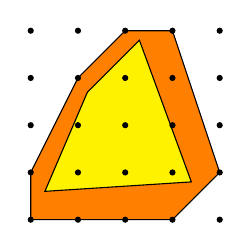
\begin{tikzpicture}[scale=0.6]
	\filldraw[fill=orange] (0,0) -- (0,1) -- (1,3) -- (2,4) -- (3,4) -- (4,1) -- (3,0) --cycle;
	\filldraw[fill=yellow] (0.3,0.6) -- (3.4,0.8) -- (2.3,3.8) --(1.2,2.7) -- cycle;
	\foreach \x in {0,...,4}
	\foreach \y in {0,...,4}
	{
		\filldraw[fill=black] (\x,\y) circle (1.5pt);
	}
	% \draw (1,0) -- (0,1) -- (2,2) --cycle;
	\end{tikzpicture}
\end{center}

This approach is still possible. It is requested by the option
\begin{itemize}
	\itemtt [Approximate, -r]
\end{itemize}

This is often a good choice, especially in low dimension.

It is not advisable to use approximation for polytopes with a large number of vertices since it must be expected that the approximation multiplies the number of vertices by $\dim P+1$ so that it may become difficult to compute the triangulation.

Approximation requires that the grading denominator is equal to $1$. If this condition is not satisfied, primal mode is used.

\subsubsection{Lattice points by the dual algorithm}

Often the dual algorithm is extremely fast. But it can also degenerate terribly. It is very fast for \verb|6x6.in| run with \verb|-d1|. The primal algorithm or approximation fail miserably. (\verb|-1|, the default choice project-and-lift, is also quite good. The difference is that \verb|-d1| does not compute the vertices that in this case are necessary for the preparation of project-and-lift.)

On the other hand, the dual algorithm is hopeless already for the $2$-dimensional parallelotope \verb|ChF_2_64.in|. Try it. It is clear that complicated arithmetic is dangerous for the dual algorithm. (The dual algorithm successively computes the lattice points correctly for all intermediate polyhedra, defined as intersections of the half spaces that have been processed so far. The intermediate polyhedra can be much more difficult than the final polytope, as in this case.)

In certain cases (see Section~\ref{div_labor}) Normaliz will try the dual algorithm if you forbid project-and-lift by \verb|NoProjection|.

\subsubsection{Counting lattice points}\label{Counting}

In some applications one is not interested in the lattice points, but only in their number. In this case you can set the computation goal
\begin{itemize}
	\itemtt [NumberLatticePoints]
\end{itemize}
The main advantage is that it does not store the lattice points and therefore cannot fail because of lack of memory if their number becomes very large. In the inhomogeneous case \verb|NumberLatticePoints| can be combined with \verb|HilbertSeries|. Then the lattice points are counted by degree. See Section~\ref{count} for an application.

\verb|NumberLatticePoints| uses project-and-lift (with floating point if \verb|ProjectionFloat| is set). Therefore don't block it. If the number of lattice points is so large that memory becomes a problem, then the primal and the dual algorithm will most likely not be able to compute them.

\subsubsection{A single lattice oint}\label{single_latt_point}

One can ask for a single lattice point by 
\begin{itemize}
	\itemtt [SingleLatticePoint]
\end{itemize}
It forces the project-and-lift algorithm. This is useful if one wants to test the solubility of a system of constraints, especially if there might be enormously many solutions in the positive case. In the negative case it does not save time.

\subsection{The bottom decomposition}\label{bottom_dec}

The triangulation size and the determinant sum of the triangulation are critical size parameters in Normaliz computations. Normaliz always tries to order the generators in such a way that the determinant sum is close to the minimum, and on the whole this works out well. The use of the bottom decomposition by \verb|BottomDecomposition, -b| enables Normaliz to compute a triangulation with the optimal determinant sum for the given set of generators, as we will explain in the following.

The determinant sum is independent of the order of the generators of the cone $C$ if they lie in a hyperplane $H$. Then the determinant sum is exactly the normalized volume of the polytope spanned by $0$ and $C\cap H$. The triangulation itself depends on the order, but the determinant sum is constant.
\begin{center}
	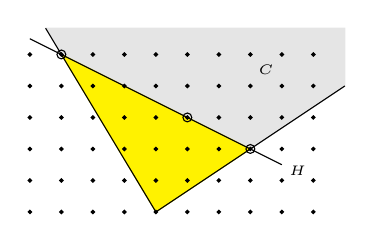
\begin{tikzpicture}[scale=0.4]
	\filldraw[gray!20] (-3.5,5.833) -- (0,0) -- (6,4) -- (6,5.833) -- cycle;
	\filldraw[yellow] (0,0) -- (-3,5) -- (3,2) -- cycle;
	\draw (-3.5,5.833) -- (0,0) -- (6,4);
	\foreach \x in {-4,...,5}
	\foreach \y in {0,...,5}
	{
		\filldraw[fill=black] (\x,\y) circle (1.5pt);
	}
	\draw (-4,5.5) --(4,1.5) node at (4.5,1.3){\tiny $H$};
	
	\draw (-3,5) circle (4pt) node at (3.5,4.5){\tiny $C$};
	\draw (1,3) circle (4pt);
	\draw (3,2) circle (4pt);
	\end{tikzpicture}
\end{center}

This observation helps to find a triangulation with minimal determinant sum in the general case.
We look at the \emph{bottom} (the union of the compact faces) of the polyhedron generated by $x_1,\dots,x_n$ as vertices and $C$ as recession cone, and take the volume underneath the bottom:
\begin{center}
	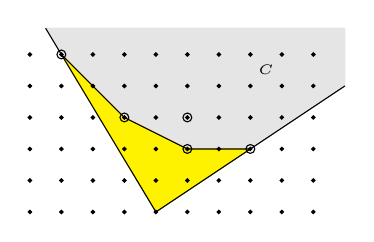
\begin{tikzpicture}[scale=0.4]
	\filldraw[gray!20] (-3.5,5.833) -- (0,0) -- (6,4) -- (6,5.833) -- cycle;
	\filldraw[yellow] (0,0) -- (-3,5) -- (-1,3) -- (1,2) -- (3,2) -- cycle;
	
	\draw (-3,5) -- (-1,3) -- (1,2) -- (3,2);
	
	\draw (-3.5,5.833) -- (0,0) -- (6,4);
	\foreach \x in {-4,...,5}
	\foreach \y in {0,...,5}
	{
		\filldraw[fill=black] (\x,\y) circle (1.5pt);
	}
	
	\draw (-3,5) circle (4pt) node at (3.5,4.5){\tiny $C$};
	\draw (-1,3) circle (4pt);
	\draw (1,3) circle (4pt);
	\draw (3,2) circle (4pt);
	\draw (1,2) circle (4pt);
	\end{tikzpicture}
\end{center}
With the option \texttt{BottomDecomposition}, \texttt{-b}, Normaliz computes a triangulation that respects the bottom facets. This yields the optimal determinant sum for the given generators. If one can compute the Hilbert basis by the dual algorithm, it can be used as input, and then one obtains the absolute bottom of the cone, namely the compact facets of the convex hull of all nonzero lattice points.

Normaliz does not always use the bottom decomposition by default since its computation requires some time and administrative overhead. However, as soon as the input ``profile'' is considered to be ``rough'' it is invoked. The measure of roughness is the ratio between the maximum degree (or $L_1$ norm without a grading) and the minimum. A ratio $\ge 10$ activates the bottom decomposition.

If you have the impression that the bottom decomposition slows down your computation, you can suppress it by 
\begin{itemize}
\itemtt[NoBottomDec, -o]
\end{itemize}

The bottom decomposition is part of the subdivision of large simplicial cones discussed in the next section.

The example \verb|strictBorda.in| belongs to social choice theory like \verb|Condorcet.in| (see Section~\ref{Condorcet}), \verb|PluralityVsCutoff.in| and \verb|CondEffPlur.in|. The last two profit enormously from symmetrization (see Section~\ref{symmetrize}), but \verb| strictBorda.in| does not. Therefore we must compute the Hilbert series for a monoid in dimension $24$ whose cone has $6363$ extreme rays. It demonstrates the substantial gain that can be reached by bottom decomposition. Since the roughness is large enough, Normaliz chooses bottom decomposition automatically, unless we block it.
\begin{center}
	\begin{tabular}{|c|r|r|}\hline
		algorithm	& triangulation size& determinant sum \\ \hline
		bottom decomposition& $30,399,162,846$ & $75,933,588,203$ \\ \hline
		standard order of extreme rays, \ttt{-o} & $119,787,935,829$ & $401,249,361,966$ \\ \hline
	\end{tabular}
\end{center}

\subsection{Subdivision of large simplicial cones}\label{subdiv}

Especially in computations with rational polytopes one encounters very large determinants that can keep the Normaliz primal algorithm from terminating in reasonable time. As an example we take \verb|hickerson-18.in| from the LattE distribution~\cite{LatInt}. It is simplicial and the complexity is totally determined by the large determinant $\approx 4.17\times 10^{14}$ (computed with \verb|-v|).

If we are just interested in the degree $1$ points, Normaliz uses the project-and-lift method of Section~\ref{project} and finds $44$ degree $1$ points in the blink of an eye. If we use these points together with the extreme rays of the simplicial cone, then the determinant sum decreases to $\approx 1.3\times 10^{12}$, and the computation of the Hilbert basis and the Hilbert series is in reach. But it is better to pursue the idea of subdividing large simplicial cones systematically. Normaliz
uses its own algorithm for finding optimal subdivision points, based on project-and-lift(and LLL reduced coordinates).

Normaliz tries to subdivide a simplicial cone if it has determinant $\ge 10^8$ or $10^7$ if the Hilbert basis is computed. Both methods are used recursively via stellar subdivision until simplicial cones with determinant $< 10^6$ have been reached or no further improvement is possible. All subdivision points are then collected, and the start simplicial cone is subdivided with bottom decomposition, which in general leads to substantial further improvement.

The following table contains some performance data for subdivisions based on the Normaliz method (default mode, parallelization with~$8$~threads).
\begin{center}
	\setlength{\tabcolsep}{3.2pt}
	\renewcommand{\arraystretch}{1.2}
	\begin{tabular}{|c|c|c|c|}
		\hline
		& \ttt{hickerson-16} & \ttt{hickerson-18} & \ttt{knapsack\_11\_60}  \\ \hline
		simplex volume & $9.83\times 10^7$ & $4.17\times 10^{14}$ & $2.8\times 10^{14}$ \\ \hline
		stellar determinant sum & $3.93\times 10^6$  & $9.07\times 10^8$  & $1.15\times 10^8$\\ \hline
		volume under bottom  & $8.10\times 10^5$ & $3.86\times 10^7$ & $2.02\times 10^7$ \\ \hline
		volume used     & $3.93\times 10^6$ & $6.56\times 10^7$ & $2.61\times 10^7$ \\ \hline
		%improvement factor & $25$ &  $7.62\times10^6$ & $1.17\times 10^7$\\ \hline
		runtime without subdivision   &  $2.8$~s & $>12$~d &  $>8$~d \\ \hline
		runtime with subdivision    &  $0.4$~s & $24$~s & $5.1$~s \\ \hline
	\end{tabular}
\end{center}

A good nonsimplicial example showing the subdivision at work is \verb|hickerson-18plus1.in| with option \verb|-q|.

Note: After subdivision the decomposition of the cone may no longer be a triangulation in the strict sense, but a decomposition that we call a \emph{nested triangulation}; see Section~\ref{nested}. If the creation of a nested triangulation must be blocked, one uses the option \verb|NoSubdivision|. Inevitably it blocks the subdivision of large simplicial cones.

\emph{Remark}\enspace The bounds mentioned above work well up to dimension $\approx 10$. For a fixed determinant, the probability for finding a subdivision point decreases rapidly.

\subsection{Primal vs.\ dual -- division of labor}\label{div_labor}

%\subsection{Normaliz tries to be smart}\label{smart}

As already mentioned several times, Normaliz has two main algorithms for the computation of Hilbert bases, the primal algorithm and the dual algorithm. It is in general very hard to decide beforehand which of the two is better for a specific example. Nevertheless Normaliz tries to guess, unless \verb|PrimalMode|, \verb|-P| or \verb|DualMode|, \verb|-d| is explicitly chosen by the user. In first approximation one can say that the dual algorithm is chosen if the computation is based on constraints and the number of inequalities is neither too small nor too large. Normaliz chooses the dual algorithm if at the start of the Hilbert basis computation the cone is defined by $s$ inequalities such that
$$
r+\frac{50}{r} \le s \le 2e
$$
where $r$ is the rank of the monoid to be computed and $e$ is the dimension of the space in which the data are embedded. These conditions are typically fulfilled for diophantine systems of equations whose nonnegative solutions are asked for.
In the case of very few or many hyperplanes Normaliz prefers the primal algorithm. While this combinatorial condition is the only criterion for Normaliz, it depends also on the arithmetic of the example what algorithm is better. At present Normaliz makes no attempt to measure it in some way.

When both Hilbert basis and Hilbert series are to be computed, the best solution can be the combination of both algorithms. We recommend \verb|2equations.in| as a demonstration example which combines the algorithmic variant \verb|DualMode| and the computation goal \verb|HilbertSeries|:
\begin{Verbatim}
amb_space 9
equations 2
1 6 -7 -18 25 -36 6 8 -9
7 -13 15 6 -9 -8 11 12 -2
total_degree
DualMode
HilbertSeries
\end{Verbatim}
As you will see, the subdivision of large simplicial cones is very useful for such computations.

Compare \verb|2equations.in| and \verb|2equations_default.in| for an impression on the relation between the algorithms.

\subsection{Various volume versions}\label{VariousVolumes}

Normaliz offers various algorithms for the volume of a polytope. They all compute the lattice normalized volume, and additionally convert it to the Euclidean volume. There are $3$ basic algorithms:
\begin{arab}
\item the \emph{primal} volume algorithm: Normaliz computes a lexicograhic triangulation, and finds the volume as the sum of the volumes of the simplices in the triangulation;
\item volume by \emph{descent in the face lattice}: there is a reverse lexicographic triangulation  in the background, but it is not computed explicitly;
\item volume by \emph{signed decomposition}: Normaliz computes a triangulation of the dual cone and converts it into a signed decomposition of the polytope.
\end{arab}

For algebraic polytopes only (1) is implemented at present. But (3) could be extended to them, whereas (2) is not suitable.

By rule of thumb one can say that  the best choice is
\begin{arab}
\item if the polytope has few vertices, but potentially many facets;
\item  if the number of vertices and the number of facets are of the same order of magnitude;
\item  if there are \emph{very} few facets and many vertices.
\end{arab}
Normaliz tries to choose the optimal algorithm by default. We will illustrate this recommendation by examples below.

There are variants:
\begin{enumerate}
\item[(a)] exploitation of isomorphism types of faces in the descent algorithm;
\item[(b)] symmetrization (explained in Section \ref{symmetrize}).
\end{enumerate}

In volume computations that are not part of a Hilbert series computation Normaliz checks the default conditions of the algorithms in the order
\begin{center}
signed decomposition $\to$  descent  $\to$ symmetrization
\end{center}
If the default conditions are not satisfied for any of them, the primal triangulation algorithm is used. These decisions must often be made on the basis of partial information. For example, the really critical parameter for descent is the number of non-simplicial facets. Therefore it can be useful to ask for a certain variant explicitly or to exclude the others. The exploitation of isomorphism types must always be asked for explicitly by the user.

Normaliz recognizes parallelotopes and applies an extremely fast method for their volumes.

We compare computation times for some significant examples in Section \ref{vvv_compare}. Normaliz always computes multiplicities of monoids, but we simply talk of volumes in this section.

\subsubsection{The primal volume algorithm}

It has been used many times in the examples of this manual, and mathematically there is nothing to say: if a polytope $P$ is decomposed into simplices with non-overlapping interiors, then its volume is the sum of the volumes of the simplices forming the decomposition.
\begin{center}
	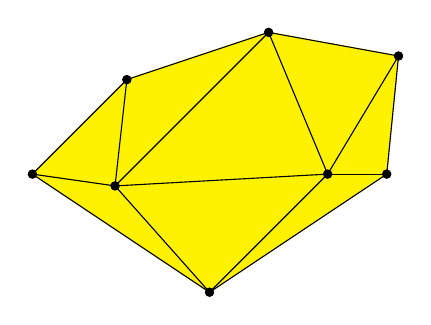
\begin{tikzpicture}[scale=1.5]
	\filldraw[color=yellow] (0,0) -- (1.5,1) -- (1.6,2) -- (0.5,2.2) -- (-0.7,1.8) -- (-1.5,1) -- cycle;
	\draw (0,0) -- (1.5,1) -- (1.6,2) -- (0.5,2.2) -- (-0.7,1.8) -- (-1.5,1) -- cycle;
	\filldraw[fill=black] (0,0)  circle (1pt);
	\filldraw[fill=black] (1.5,1)  circle (1pt);
	\filldraw[fill=black] (1.6,2)  circle (1pt);
	\filldraw[fill=black] (0.5,2.2)  circle (1pt);
	\filldraw[fill=black] (-0.7,1.8)  circle (1pt);
	\filldraw[fill=black] (-1.5,1)  circle (1pt);
	\filldraw[fill=black] (1,1)  circle (1pt);
	\filldraw[fill=black] (-0.8,0.9)  circle (1pt);
	\draw (1,1) --  (-0.8,0.9);
	\draw (-1.5,1) --  (-0.8,0.9);
	\draw (0,0) --  (-0.8,0.9);
	\draw (1,1) --  (0,0);
	\draw (1,1) --  (1.6,2);
	\draw (1,1) --  (1.5,1);
	\draw (1,1) --  ((0.5,2.2);
	\draw (-0.8,0.9) --  (0.5,2.2);
	\draw (-0.8,0.9) --  (-0.7,1.8);
	\end{tikzpicture}
\end{center}

\subsubsection{Volume by descent in the face lattice}\label{descent}

The idea is to exploit the formula
$$
\operatorname{mult}(P)=\sum_i \operatorname{ht}_{F_i}(v)\operatorname{mult}(F_i)/\deg(v).
$$
recursively where $v$ is a vertex of the polytope $P$ with as few opposite facets $F_i$ as possible, and $\operatorname{ht}_{F_i}(v)$ is the lattice height of $v$ over $F_i$. The formula is illustrated by the figure:
\begin{center}
	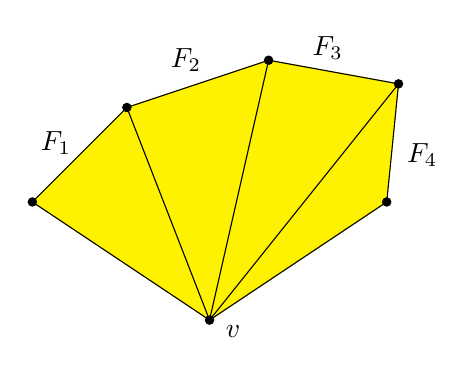
\begin{tikzpicture}[scale=1.5]
	\filldraw[color=yellow] (0,0) -- (1.5,1) -- (1.6,2) -- (0.5,2.2) -- (-0.7,1.8) -- (-1.5,1) -- cycle;
	\draw (0,0) -- (1.5,1) -- (1.6,2) -- (0.5,2.2) -- (-0.7,1.8) -- (-1.5,1) -- cycle;
	\draw (0,0) -- (0.5,2.2);
	\draw (0,0) -- (1.6,2);
	\draw (0,0) -- (-0.7,1.8);
	\draw node at (0.2,-0.1){$v$};
	\filldraw[fill=black] (0,0)  circle (1pt);
	\filldraw[fill=black] (1.5,1)  circle (1pt);
	\filldraw[fill=black] (1.6,2)  circle (1pt);
	\filldraw[fill=black] (0.5,2.2)  circle (1pt);
	\filldraw[fill=black] (-0.7,1.8)  circle (1pt);
	\filldraw[fill=black] (-1.5,1)  circle (1pt);
	\draw node at (-1.3,1.5){$F_1$};
	\draw node at (-0.2,2.2){$F_2$};
	\draw node at (1.0,2.3){$F_3$};
	\draw node at (1.8,1.4){$F_4$};
	\end{tikzpicture}
\end{center}
The recursive application results  in building a subset $\mathcal F$ of the face lattice so that for each face $F\in\mathcal F$ to which the formula is applied all facets of $F$ that are opposite to the selected vertex are contained in $\mathcal F$. However, if a face is simplicial, its multiplicity is computed by the standard determinant formula. The algorithm is implemented in such a way that all data are collected in the descent and no backtracking is necessary. The RAM usage is essentially determined by the two largest layers. For a detailed discussion we refer the reader to \cite{BI2}. However, meanwhile many examples disussed in \cite{BI2} can be computed much faster by signed decomposition, which is discussed below.

You can force this algorithm is by
\begin{itemize}
	\itemtt[Descent, -F]
\end{itemize}
and block it by
\begin{itemize}
	\itemtt[NoDescent]
\end{itemize}
Note that \verb|Descent| does \emph{not} imply \verb|Multiplicity| or \verb|Volume|. (We cannot exclude that in the future descent is used also for other computations.)

As an example we have a look at \ttt{lo6} and show part of its terminal output. We look at this example again when we discuss the variant that exploits isomorphism types.
\begin{Verbatim}
Command line: -c ../example/lo6 -iv --Descent 
Compute: Multiplicity Descent 
...
Descent from dim 15, size 854
..................................................
Descent from dim 14, size 7859
..................................................
Descent from dim 13, size 37587

\end{Verbatim}

\subsubsection{Descent exploiting isomorphism classes of faces}\label{ExploitIsosoMult}

The descent algorithm computes a subset of the face lattice. We can reduce the size of this ``descent system'' if we identify faces in it that are isomorphic. In order to have a beneficial effect on computation time, the reduction must be substantial since the computation of isomorphism types is relatively slow. The polytope should at least have a large automorphism group, but this alone is no guarantee for an acceleration. The exploitation of isomorphism types is asked for by
\begin{itemize}
	\itemtt[Descent ExploitIsosMult]
\end{itemize}
It is better to ask for \ttt{Descent} explicitly, but \ttt{ExploitIsosMult} will be recognized if \ttt{Descent} is chosen by default.

This variant is only available if Normaliz has been built with nauty and hash-library. The latter is used to store the normal forms that take much memory by their SHA256 hash values. But you can insist on strict type checking by
\begin{itemize}
	\itemtt[StrictIsoTypes]
\end{itemize}

We show a little bit of the terminal output for \ttt{lo6} for which this variant is particularly fast:
\begin{Verbatim}
Command line: -c ../example/lo6 -iv --Descent --ExploitIsosMult 
Compute: Multiplicity Descent ExploitIsosMult 
...
Descent from dim 15, size 2
Descent from dim 14, size 232
Collecting isomorphism classes
..................................................
Iso types 5
Descent from dim 13, size 224
Collecting isomorphism classes
...
\end{Verbatim}
Compared to \ttt{Descent} without exploitation of isomorphism classes the reduction is indeed substantial, and is reflected drastically by the computation times.

Using isomorphism types opens descent for polytopes with many facets, but few isomorphism classes of them.

\subsubsection{Volume by signed decomposition}

This algorithm uses that a ``generic'' triangulation of the dual cone induces a ``signed decomposition'' of the primal polytope. More precisely: the indicator function of the primal polytope is the sum of the indicator functions of simplices with appropriate signs.

 Let $P\subset \RR^d$ be a polytope of dimension $d$ (it is important that $P$ is full-dimensional). We realize $P$ as the intersection of a cone $C$ with the hyperplane $H$ defined by a grading $\gamma$: $H=\{x:\gamma(x)=1\}$. The grading is an interior element of the dual cone $C^*=\{\lambda\in(\RR^d)^*:\lambda(x)\ge 0 \text { for all }x\in C  \}$. In order to visualize the situation we take an auxiliary (irrelevant) cross-section $Q$ of the dual cone:
 \begin{center}
 	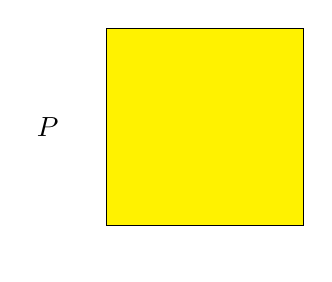
\begin{tikzpicture}[scale=2.5]
 	\filldraw[color=yellow] (0,0) -- (1,0) -- (1,1) -- (0,1) -- cycle;
 	\draw (0,0) -- (1,0) -- (1,1) -- (0,1) -- cycle;
 	\draw node at (-0.3,0.5){$P$};
 	\draw node at (0,-0.1){};
 	\end{tikzpicture}
 	\qquad\qquad
  	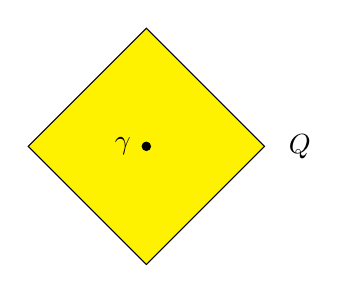
\begin{tikzpicture}[scale=1.5]
	 \filldraw[color=yellow] (1,0) -- (0,1) -- (-1,0) -- (0,-1) -- cycle;
 	 \draw (1,0) -- (0,1) -- (-1,0) -- (0,-1) -- cycle;
  	\draw node at (1.3,0){$Q$};
   	\filldraw (0,0) circle (1pt);
  	\draw node at (-0.2,0){$\gamma$};
 \end{tikzpicture}
 \end{center}
 
 Now suppose that we have a \emph{generic} triangulation $\Delta$ of the dual cone where genericity is defined as follows: $\gamma$ is not contained in any hyperplane that intersects any $\delta\in\Delta$ in a facet. Let $\delta\in\Delta$ be given, and denote the linear forms on $(\RR^d)^*$ defining its facets by $\ell_1,\dots\ell_d\in (\RR^d)^{**} = \RR^d$. ( $\ell_1,\dots\ell_d$ are the extreme rays of the dual of $\delta$.) The hyperplanes defined by the vanishing of $\ell_1,\dots\ell_d$ decompose $(\RR^d)^*$ into ``orthants'' that can be labeled by a sign vector $\sigma=(s_1,\dots,s_d)\in \{ \pm 1  \}^d$:
 $$
 D(\delta,\sigma)=\{\alpha: (-1)^{s_i} \ell_i(\alpha) \ge 0   \}.
 $$
 By the assumption on $\gamma$, there is \emph{exactly on}e sign vector $\sigma$ such that $\gamma $  lies in the interior of $ D(\delta,\sigma)$. Consequently the hyperplane $H$ intersects the dual  $D(\delta,\sigma)^*$ in a polytope $R_\delta$. (We identify $(\RR^d)^{**}$ with $\RR^d$.) Furthermore we set $e(\delta)=|\{i: s_i=-1 \}|$.
 
 Let $\iota_X$ denote the indicator function of a subset $X\subset \RR^d$. Then
 \begin{equation}
 \iota_P(x) = \sum_{\delta\in \Delta} (-1) ^{e(\delta)} \iota_{R_\delta}(x)\label{iota}
 \end{equation}
 for all $x\in\RR^d$ outside a union of finitely many hyperplanes. Since volume (lattice normalized or Euclidean) is additive on indicator functions this formula can be used for the computation of the volume of $P$. (We give a reference at the end of this section.)
 
 In order to find a generic triangulation, Normaliz first computes a triangulation $\Delta_0$ of $C^*$ and saves the induced ``hollow triangulation'' that $\Delta_0$ induces on the boundary of $C^*$. Then it finds a ``generic'' element $\omega\in C^*$ such that the ``star'' triangulation $\Delta$ of $C^*$ in which every simplicial cone is the pyramid with apex $\omega$ and base in the hollow triangulation is generic. 
 \begin{center}
 	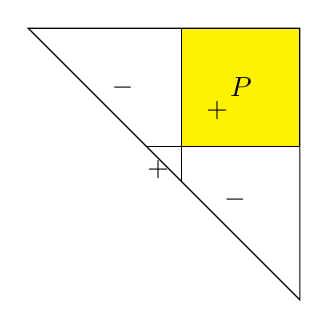
\begin{tikzpicture}[scale=1.5]
 	\filldraw[color=yellow] (0,0) -- (1,0) -- (1,1) -- (0,1) -- cycle;
 	\draw (0,0) -- (1,0) -- (1,1) -- (0,1) -- cycle;
 	\draw node at (0.5,0.5){$P$};
 	\draw node at (0,-0.1){};
    \draw (-1.3,1) -- (1,1) -- (1,-1.3) -- cycle;
    \draw (1,0) -- (-0.3,0);
    \draw (0,1) -- (0,-0.3);
    \draw node at (0.3,0.3){$+$};
    \draw node at (-0.5,0.5){$-$};
    \draw node at (0.45,-0.45){$-$};
    \draw node at (-0.2,-0.2){$+$};
 	\end{tikzpicture}
 	\qquad\qquad
 	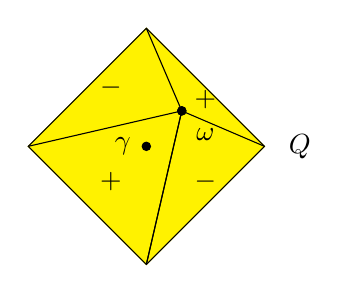
\begin{tikzpicture}[scale=1.5]
 	\filldraw[color=yellow] (1,0) -- (0,1) -- (-1,0) -- (0,-1) -- cycle;
 	\draw (1,0) -- (0,1) -- (-1,0) -- (0,-1) -- cycle;
 	\draw node at (1.3,0){$Q$};
 	\filldraw (0,0) circle (1pt);
 	\draw node at (-0.2,0){$\gamma$};
  	\filldraw (0.3,0.3) circle (1pt);
  	\draw (-1,0) -- (0.3,0.3) -- (0,1);
  	\filldraw (0.3,0.3) circle (1pt);
  	\draw (1,0) -- (0.3,0.3) ;
  	\draw (0,-1) -- (0.3,0.3) ;
    \draw (0,-1) -- (0.3,0.3) ;
  	\draw node at (0.5,0.1){$\omega$};
    \draw node at (-0.3,-0.3){$+$}; 
    \draw node at (0.5,0.4){$+$};
    \draw node at (-0.3,0.5){$-$};  
    \draw node at (0.5,-0.3){$-$};	
 	\end{tikzpicture}
 \end{center} 

 Since $\omega$ almost  inevitably has unpleasantly large coordinates, the polytopes $R_\delta$ have even worse rational vertices, and their volumes usually are rational numbers with very large numerators and denominators. This extreme arithmetical complexity limits the applicability of the signed decomposition. 
 
Signed decomposition is asked for by
\begin{itemize}
	\itemtt[SignedDec]
\end{itemize}
and blocked by
\begin{itemize}
	\itemtt[NoSignedDec]
\end{itemize}

We show part of the terminal output for \ttt{strictBorda}: 
 \begin{Verbatim}
...
Command line: -c ../example/strictBorda 
Compute: Multiplicity 
Working with dual cone
************************************************************
starting full cone computation
Starting primal algorithm with full triangulation ...
...
Computing  by signaed decomposition
Making hollow triangulation
...
Size of triangulation 100738
Size of hollow triangulation 324862
Trying to find geric vector
Trying to find generic linear combination of 
164 107 65 125 116  66 ...  100
32 130 57 105 108 153 ...  139
...
Must increase coefficients
Trying to find generic linear combination of 
270 228 347 407 399 280 ...167
227 362 305 135 354 272 ... 499

Generic with coeff 56 1
Computing multiplicity
Generic 15347 13130 19737 22927 ...9851 
...

Mult (before ...) 1281727528...66511/25940255...784000000000
Mult (float) 4.94107527277e-05
 \end{Verbatim}
 
 The algorithm described in this section has been developed by Lawrence \cite{Lawrence} in the language of linear programming, and \cite{practical} describes the floating point implementation in  the package vinci \cite{vinci}. We have learnt it from Filliman's paper \cite{Filli}, which contains a proof of equation \eqref{iota}. See also the references to older literature in \cite{Filli}.
 
 Volume by signed decomposition allows distributed computing. See Appemdix \ref{distr_comp}.
 
 \subsubsection{Fixed precision for signed decomposition}\label{FixedPrecision}
 
 In very large computations the fractions that arise in the computation of volumes by signed decomposition can become gigantic (indeed, take gigabytes) so that their handling becomes impossible. Therefore Normaliz has a fixed precision option for volumes by signed decomposition. This means that the volumes of the simplices in the hollow triangulation are computed precisely as rational numbers, but are truncated to fixed precision before being added.
The cone property to be used is
  \begin{itemize}
 	\itemtt[FixedPrecision]
 \end{itemize}
It defines the precision to be $10^{-100}$. Then the precision of the final result is $\le H*10^{-100}$ where $H$ is the number of simplices in the hollow triangulation. Therefore $10^{-100}$ should suffice for all computations that can be done at present.
 
 If the default value of $100$ is too large or too small it can be set by
 \begin{itemize}
 	\itemtt[decimal\_digits <n>]
 \end{itemize}
in the input file.

We run \verb|strictBorda_fixed_prec.in|:
\begin{Verbatim}
amb_space 24
inequalities 9
...
Multiplicity
FixedPrecision
\end{Verbatim}
Then the terminal output ends by
\begin{Verbatim}
Mult (before NoGradingDenom correction) 4941075272...6309/1000000...000000000
Mult (float) 4.94107527277e-05
\end{Verbatim}
and in the output file we find
\begin{Verbatim}
multiplicity (fixed precision) = 4941075...1726309/100000000...00000000000
multiplicity (float) = 4.94107527277e-05
\end{Verbatim}

\subsubsection{Comparing the algorithms}\label{vvv_compare}

The computation times in the table were obtained on a compute server with a parallelization of $32$ threads in order to save time for the big computations. The fast ones do not really profit from it. The optimal time is printed in bold face. If the default choice is different, it is indicted in italics.

\begin{footnotesize}
\begin{tabular}{l|r|r|r|r|r|r|r|r|r|}
& dim & $\#$ext & $\#$supp & signed dec&desc iso&descent& symm & symm sd& primal\\
\hline
\ttt{A553} & 43 &75&306955&--&\textbf{5:48 m}&--&--&--&\emph{45:35 m}\\
\hline
\ttt{lo6}&16&720&910& --   & \textbf{6.0 s}& 2:16 m & -- & --& \emph{18:07 m}\\
\hline
\ttt{cross-24}&25&48&$2^{24}$ & -- & 7:59 m &10:43 m & -- & --& \textbf{7:55 m}\\
\hline
\ttt{CondEffPlur}&24&3928&30& \textbf{0.3 s }&2.5 s & 0.9 s & 6:28 m & 31.3 s & 41 h \\
\hline
\ttt{strictBorda}&24&6363& 33 & \textbf{2.0 s} & -- & 26.7 s& -- & -- & 4:18 h \\
\hline
\end{tabular}
\end{footnotesize}

The decision for \ttt{lo6} is made without knowledge of the unexpectedly small number of support hyperplanes. This is a design decision of Normaliz: if the primal algorithm should apply, then it would be time consuming to compute the support hyperplanes beforehand. But in this case it is the wrong decision. 

For \ttt{A553} it is unpredictable that descent with isomorphism types speeds up the computation of the volume -- one would have at least to compute the automorphism group and see that the number of orbits of the support hyperplanes is really small.

One would expect that descent with isomomorphism types is very fast for \ttt{cross-24} since there is single orbit of support hyperplanes. But it takes time to find this out, and the primal algorithm is slightly faster.

\ttt{CondEffPlur} illustrates the evolution of volume computations in Normaliz. Though symmetrization is not the fastest choice for any of the examples in the table, it remains important since we have no better algorithm for the computation of the Hilbert series of \ttt{CondEffPlur} and related examples.

\subsection{Checking the Gorenstein property}\label{Gorenstein}

If the Hilbert series has been computed, one can immediately see whether the monoid computed by Normaliz is Gorenstein: this is the case if and only if the numerator is a symmetric polynomial, and Normaliz indicates that (see Section~\ref{job_dual}). However, there is a much more efficient way to check the Gorenstein property, which does not even require the existence of a grading: we must test whether the \emph{dual} cone has degree $1$ extreme rays. This amounts to checking the existence of an implicit grading on the dual cone.

This very efficient Gorenstein test is activated by the option \ttt{IsGorenstein}, equivalently \ttt{-G} on the command line. We take \verb|5x5Gorenstein.in|:

\begin{Verbatim}
amb_space 25
equations 11
1 1 1 1 1 -1 -1 -1 -1 -1  0  0  0  0  0  0  0  0  0  0  0  0  0  0  0
...
1 1 1 1 0  0  0  0 -1  0  0  0 -1  0  0  0 -1  0  0  0 -1  0  0  0  0
IsGorenstein
\end{Verbatim}

In the output we see
\begin{Verbatim}
Monoid is Gorenstein 
Generator of interior
1 1 1 1 1 1 1 1 1 1 1 1 1 1 1 1 1 1 1 1 1 1 1 1 1 
\end{Verbatim}

In fact, the Gorenstein property is (also) equivalent to the fact that the interior of our monoid is generated by a single element as an ideal, and this generator is computed if the monoid is Gorenstein. (It defines the grading under which the extreme rays of the dual cone have degree~$1$.)

If the monoid is not Gorenstein, Normaliz will print the corresponding message.

\subsection{Symmetrization}\label{symmetrize}

Under certain conditions one can count lattice points in a cone $C$ by mapping $C$ to a cone $C'$ of lower dimension and then counting each lattice point $y$ in $C'$ with the number of its lattice preimages. This approach works well if the number of preimages is given by a polynomial in the coordinates of $y$. Since $C'$ has lower dimension, one can hope that its combinatorial structure is much simpler that that of $C$. One must of course pay a price: instead of counting each lattice point with the weight $1$, one must count it with a polynomial weight. This amounts to a computation of a weighted Ehrhart series that we will discuss in Section~\ref{Poly_comp}. Similarly multiplicity can be computed as the virtual multiplicity of a polynomial after projection.

The availability of this approach depends on symmetries in the coordinates of $C$, and therefore we call it \emph{symmetrization}. Normaliz tries symmetrization under the following condition: $C$ is given by constraints (inequalities, equations, congruences, excluded faces) and the inequalities contain the sign conditions $x_i\ge 0$ for all coordinates $x_i$ of $C$. (Coordinate hyperplanes may be among the excluded faces.) Then Normaliz groups coordinates that appear in all constraints and the grading (!) with the same coefficients, and, roughly speaking, replaces them by their sum. The number of preimages that one must count for the vector $y$ of sums is then a product of binomial coefficients -- a polynomial as desired. More precisely, if $y_j$, $j=1,\dots,m$, is the sum of $u_j$ variables $x_i$ then
$$
f(y)=\binom{u_1+y_1-1}{u_1-1}\cdots \binom{u_m+y_m-1}{u_m-1}.
$$
is the number of preimages of $(y_1,\dots,y_m)$. This approach to Hilbert series has been suggested by A.~Sch\"urmann~\cite{Sch}.

Note that symmetrization requires an explicit grading. Moreover, it sets \verb|NoGradingDenom|.

As an example we look again at the input for the Condorcet paradox:
\begin{Verbatim}
amb_space 24
inequalities 3
1 1 1 1 1 1 -1 -1 -1 -1 -1 -1   1  1 -1 -1  1 -1   1  1 -1 -1  1 -1
1 1 1 1 1 1  1  1 -1 -1  1 -1  -1 -1 -1 -1 -1 -1   1  1  1 -1 -1 -1
1 1 1 1 1 1  1  1  1 -1 -1 -1   1  1  1 -1 -1 -1  -1 -1 -1 -1 -1 -1
nonnegative
total_degree
Multiplicity
\end{Verbatim}
The grading is completely symmetric, and it is immediately clear that the input is symmetric in the first $6$ coordinates. But also the column of three entries $-1$ appears $6$ times, and there are $6$ more groups of $2$ coordinates each (one group for each $\pm1$ pattern). With the suitable labeling, the number of preimages of$(y_1,\dots,y_8$) is given by
$$
f(y)=\binom{y_1+5}{5}(y_2+1)(y_3+1)(y_4+1)(y_5+1)(y_6+1)(y_7+1)\binom{y_8+5}{5}.
$$
Normaliz finds the groups of variables that appear with the same sign pattern, creates the data for the weighted Ehrhart series, and interprets it as the Hilbert series of the monoid defined by the input data.

However, there is a restriction. Since the polynomial arithmetic has its own complexity and Normaliz must do it in GMP integers, it makes no sense to apply symmetrization if the dimension does not drop by a reasonable amount. Therefore we require that
$$
\dim C' \le \frac{2}{3}\dim C).
$$
If called with the option \verb|-q|, Normaliz will try symmetrization, and also with \verb|-v|, provided the multiplicity has not already been computed by the descent algorithm (see Section~\ref{descent}). If the inequality for $\dim C'$ is not satisfied, it will simply compute the Hilbert series or the multiplicity without symmetrization. (In default mode it of course tries symmetrization for the Hilbert series.)

Whenever Normaliz has used symmetrization, it writes the file \verb|<project>.symm.out| that contains the data of the symmetrized object. In it you find the multiplicity of \verb|<project>.out| as virtual multiplicity and the Hilbert series as weighted Ehrhart series.

If you use the option \verb|Symmetrize|, then the behavior depends on the other options:
\begin{arab}
	\item If neither the \verb|HilbertSeries| nor \verb|Multiplicity| is to be computed, Normaliz writes only the output file \verb|<project>.symm.out| computed with \verb|SupportHyperplanes|.
	\item If one of these goals is to be computed, Normaliz will do the symmetrization, regardless of the dimension inequality above (and often this makes sense).
\end{arab}
By doing step (1) first, the user gets useful information of what to expect by symmetrization. In a second run, one can add \verb|HilbertSeries| or \verb|Multiplicity| if (1) was satisfactory.

The Condorcet example is too small in order to demonstrate the power of symmetrization. A suitable example is \verb|PluralityVsCutoff.in|:
\begin{Verbatim}
winfried@ubuntu:~/Dropbox/git_normaliz/source$ time ./normaliz -c ../example/PluralityVsCutoff
                                                    \.....|
                    Normaliz 3.3.0                   \....|
                                                      \...|
     (C) The Normaliz Team, University of Osnabrueck   \..|
                     March  2017                        \.|
                                                         \|
************************************************************
Command line: -c ../example/PluralityVsCutoff 
Compute: DefaultMode 
Embedding dimension of symmetrized cone = 6
...
------------------------------------------------------------
transforming data... done.

real	0m2.655s
user	0m5.328s
sys	0m0.080s
\end{Verbatim}
The Hilbert series is computable without symmetrization, but you better make sure that there is no power failure for the next week if you try that. (The time above includes the Hilbert basis computed automatically in dual mode).

Another good example included in the distribution is \verb|CondEffPlur.in|, but it takes some hours with symmetrization (instead of days without). For it, the dimension drops only from $24$ to $13$.

Symmetrization is a special type of computations with a polynomial weight, and therefore requires Normaliz to be built with CoCoALib.

In the computation of multiplicities via symmetrization Normaliz can use (implicitly or explicitly) signed decomposition, including fixed prrecision if asked for.

\subsection{Computations with a polynomial weight}\label{Poly_comp}

For a graded monoid $M$, which arises as the intersection $M=C\cap L$ of a rational cone$C$ and a lattice $L$, Normaliz computes the volume of
the rational polytope
$$
P=\{x\in \RR_+ M: \deg x=1\},
$$
called the multiplicity of $M$ (for the given grading), the Hilbert series of $M$, and the quasipolynomial representing the Hilbert function. This Hilbert series of $M$ is also called the Ehrhart series of $P$ (with respect to $L$), and for the generalization introduced in this section we speak of Ehrhart series and functions.

The computations of these data can be understood as integrals of the
constant polynomial $f=1$, namely with respect to the counting
measure defined by $L$ for the Ehrhart function, and with
respect to the (suitably normed) Lebesgue measure for the
volume. Normaliz generalizes these computations to
arbitrary polynomials $f$ in $n$ variables with rational
coefficients. (Mathematically, there is no need to restrict
oneself to rational coefficients for $f$.)

More precisely, set
$$
E(f,k)=\sum_{x\in M, \deg x=k} f(x),
$$
and call $E(f,\_)$ the \emph{weighted Ehrhart function} for
$f$. (With $f=1$ we simply count lattice points.) The
\emph{weighted Ehrhart series} is the ordinary generating
function
$$
E_f(t)=\sum_{k=0}^\infty E(f,k)t^k.
$$
It turns out that $E_f(t)$ is the power series expansion of a
rational function at the origin, and can always be written in
the form
$$
E_f(t)=\frac{Q(t)}{(1-t^\ell)^{\totdeg f+\rank M}},\qquad Q(t)\in\QQ[t],\
\deg Q< \totdeg f+\rank M.
$$
Here $\totdeg f$ is the total degree of the polynomial $f$, and
$\ell$ is the least common multiple of the degrees of the
extreme integral generators of $M$. See~\cite{BS} for an
elementary account, references and the algorithm used by Normaliz.

Note that \verb|excluded_faces| is a homogeneous input type. For them the monoid $M$ is replaced by the set
$$
M'=C'\cap L
$$
where $C'=C\setminus \mathcal F$ and $\mathcal F$ is the union of a set of
faces
(not necessarily facets) of $C$. What has been said above about the structure
of the weighted Ehrhart series remains true. We discuss an example below.

It follows from the general theory of rational generating
functions that there exists a quasipolynomial $q(k)$ with
rational coefficients and of degree $\le \totdeg f+\rank M-1$ that
evaluates to $E(f,k)$ for all $k\ge 0$.

Let $m=\totdeg f$ (we use this notation to distinguish the degree of the polynomial from the degree of lattice points) and $f_m$ be the degree $m$ homogeneous
component of $f$. By letting $k$ go to infinity and
approximating $f_m$ by a step function that is constant on the
meshes of $\frac 1kL$ (with respect to a fixed basis), one sees
$$
q^{(j)}_{\totdeg f+\rank M-1}=\int_P f_m\, d\lambda
$$
where $d\lambda$ is the Lebesgue measure that takes value $1$
on a basic mesh of $L\cap \RR M$ in the hyperplane of degree
$1$ elements in $\RR M$. In particular, the \emph{virtual
	leading coefficient} $q^{(j)}_{\totdeg f+\rank M-1}$ is
constant and depends only on $f_m$. If the integral vanishes,
the quasipolynomial $q$ has smaller degree, and the true
leading coefficient need not be constant. Following the
terminology of commutative algebra and algebraic geometry, we
call
$$
(\totdeg f+\rank M-1)!\cdot q_{\totdeg f+\rank M-1}
$$
the \emph{virtual multiplicity} of $M$ and $f$. It is an
integer if $f_m$ has integral coefficients and $P$ is a lattice
polytope.

The input format of polynomials has been discussed in Section~\ref{poly_input}.

The terminal output contains a factorization of the polynomial as well as some computation results. From the terminal output you may also recognize that Normaliz first computes the triangulation and the Stanley decomposition and then applies the algorithms for integrals and weighted Ehrhart series.

\emph{Remarks} \enspace (1) Large computations with many parallel threads may require much memory due to the fact that very long polynomials must be stored. Another reason for large memory usage can be the precomputed triangulation or Stanley decomposition.

(2) You should think about the option \verb|BottomDecomposition|. It will be applied to the symmetrized input. (Under suitable conditions it is applied automatically.)

(3) A priori it is not impossible that Normaliz replaces a given grading $\deg$ by $\deg/g$ where $g$ is the grading denominator. If you want to exclude this possibility, set \verb|NoGradingDenom|.


\subsubsection{A weighted Ehrhart series}

We discuss the Condorcet paradox again (and the last time), now starting from the symmetrized form. The file \ttt{Condorcet.symm.in} from the directory
\ttt{example} contains the following:

\begin{Verbatim}
amb_space 8
inequalities 3
1 -1 1 1 1 -1 -1 -1
1 1 -1 1 -1 1 -1 -1
1 1 1 -1 -1 -1 1 -1
nonnegative
total_degree
polynomial
1/120*1/120*(x[1]+5)*(x[1]+4)*(x[1]+3)*(x[1]+2)*(x[1]+1)*(x[2]+1)*
(x[3]+1)*(x[4]+1)*(x[5]+1)*(x[6]+1)*(x[7]+1)*(x[8]+5)*(x[8]+4)*
(x[8]+3)*(x[8]+2)*(x[8]+1);
\end{Verbatim}
We have seen this polynomial in Section~\ref{symmetrize} above.


From the Normaliz directory we start the computation by
\begin{Verbatim}
./normaliz -cE example/Condorcet.symm
\end{Verbatim}
We could have used \verb|--WeightedEhrhartSeries| instead of \verb|-E| or put \verb|WeightedEhrhartSeries| into the input file.

The file \ttt{Condorcet.symm.out} we find the information on the weighted Ehrhart series:

\begin{Verbatim}
Weighted Ehrhart series:
1 5 133 363 ... 481 15 6
Common denominator of coefficients: 1
Series denominator with 24 factors:
1: 1  2: 14  4: 9

degree of weighted Ehrhart series as rational function = -25

Weighted Ehrhart series with cyclotomic denominator:
...
\end{Verbatim}
The only piece of data that we haven't seen already is the common denominator of coefficients. But since the polynomial has rational coefficients, we cannot any longer expect that the polynomial in the numerator of the series has integral coefficients. We list them as integers, but must then divide them by the denominator (which is$1$ in thus case since the weighted Ehrhart series is a Hilbert series in disguise). As usual, the representation with a denominator of cyclotomic polynomials follows.

And we have the quasipolynomial as usual:

\begin{Verbatim}
Weighted Ehrhart quasi-polynomial of period 4:
0:   6939597901822221635907747840000 20899225...000000 ... 56262656
1:   2034750310223351797008092160000  7092764...648000 ... 56262656
2:   6933081849299152199775682560000 20892455...168000 ... 56262656
3:   2034750310223351797008092160000  7092764...648000 ... 56262656
with common denominator: 6939597901822221635907747840000
\end{Verbatim}

The left most column indicates the residue class modulo the period, and the
numbers in line $k$ are the coefficients of the $k$-th polynomial after
division by the common denominator. The list starts with $q_0^{(k)}$ and ends
with (the constant) $q_{23}^{(k)}$.
The interpretation of the remaining data is obvious:

\begin{Verbatim}
Degree of (quasi)polynomial: 23

Expected degree: 23

Virtual multiplicity: 1717/8192
Virtual multiplicity (float) = 0.209594726562
\end{Verbatim}

Weighted Ehrhart series can be computed for polytopes defined by homogeneous or inhomogeneous input. Weighted Ehrhart series as a weighted variant of Hilbert series for unbounded polyhedra are not defined in Normaliz.


\subsubsection{Virtual multiplicity}

Instead of the option \verb|-E| (or (\verb|--WeightedEhrhartSeries|) we use \verb|-L| or (\verb|--VirtualMultiplicity|). Then we can extract the virtual multiplicity from the output file.

The scope of computations is the same as for Weighted Ehrhart series.

\subsubsection{An integral}
In their paper \emph{Multiplicities of classical varieties} (Proc.\ Lond.\ Math.\ Soc.\ 110 (2015), no.~4, 1033--1055) J.~Jeffries, J.~Monta\~no and M.~Varbaro ask
for the computation of the integral
$$
\int\limits_{\substack{[0,1]^m \\ \sum{x}= t}}(x_1\cdots x_{m})^{n-m}\prod_{1\le i<j \le m}(x_j-x_i)^2 \mathrm d{\mu}\
$$
taken over the intersection of the unit cube in $\RR^m$ and the hyperplane of constant coordinate sum $t$. It is supposed that $t\le m \le n$. We compute the integral for $t=2$, $m=4$ and $n=6$.

The polytope is specified in the input file \ttt{j462.in} (partially typeset in $2$
columns):

\begin{Verbatim}
amb_space 5          -1 0 0 0 1   
inequalities 8       0 -1 0 0 1   
1 0 0 0 0            0 0 -1 0 1   
0 1 0 0 0            0 0 0 -1 1   
0 0 1 0 0            equations 1  
0 0 0 1 0            -1 -1 -1 -1 2
grading
unit_vector 5
polynomial
(x[1]*x[2]*x[3]*x[4])^2*(x[1]-x[2])^2*(x[1]-x[3])^2*
(x[1]-x[4])^2*(x[2]-x[3])^2*(x[2]-x[4])^2*(x[3]-x[4])^2;
\end{Verbatim}

The $8$ inequalities describe the unit cube in $\RR^4$ by the inequalities $0\le z_i\le 1$
and the equation gives the hyperplane $z_1+\dots+z_4=2$ (we must use homogenized coordinates!). (Normaliz would find the grading itself.)

From the Normaliz directory the computation is called by

\begin{Verbatim}
./normaliz -cI example/j462
\end{Verbatim}
where \verb|-I| could be replaced by \verb|--Integral|.

It produces the output in \ttt{j462.out} containing

\begin{Verbatim}
integral  = 27773/29515186701000
integral  (float) = 9.40973210888e-10
\end{Verbatim}

As pointed out above, \emph{Normaliz integrates with respect to the measure in which the basic lattice mesh has volume $1$}. (this is $1/r!$ times the lattice normalized measure, $r=\dim P$.) In the full dimensional case that is just the standard Lebesgue measure. But in lower dimensional cases this often not the case, and therefore Normaliz also computes the integral with respect to this \emph{Euclidean} measure:
\begin{Verbatim}
integral (euclidean) = 1.88194642178e-09
\end{Verbatim}

Note that \verb|Integral| automatically sets \verb|NoGradingDenom| since the polytope must be fixed for integrals.

Note: integrals can be computed by signed decomposition, and Normaliz chooses this variant if it seems better. Nevertheless you can control it by \ttt{SignedDec} and \ttt{NoSignedDec}. Fixed precision set by \verb|decimal_digits| is used for integrals as well.

\subsection{Expansion of the Hilbert or weighted Ehrhart series}\label{expansion}

Normaliz can compute the expansion of the Hilbert function or the weighted Ehrhart function up to a given degree. To this end its expands the series. For the Hilbert function there is a second possibility by lattice point computation.

\subsubsection{Series expansion}
This is best explained by \verb|CondorcetExpansion.in|:
\begin{Verbatim}
amb_space 24
inequalities 3
1 1 1 1 1 1      -1 -1 -1 -1 -1 -1   1 1 -1 -1 1 -1     1 1 -1 -1 1 -1
1 1 1 1 1 1       1 1 -1 -1 1 -1    -1 -1 -1 -1 -1 -1   1 1 1 -1 -1 -1
1 1 1 1 1 1       1 1 1 -1 -1 -1     1 1 1 -1 -1 -1    -1 -1 -1 -1 -1 -1
nonnegative
total_degree
HilbertSeries
expansion_degree 50
\end{Verbatim}
By \verb|expansion_degree 50| we tell Normaliz to compute the coefficients from degree~$0$ to degree~$50$ in the expansion of the Hilbert series. So the output contains
\begin{Verbatim}
Expansion of Hilbert series
0: 1
1: 6
2: 153
3: 586
4: 7143
5: 21450
...
49: 817397314032054600
50: 1357391110355875044
\end{Verbatim}
If the shift is nonzero, it is automatically added to the degree so that the expansion always starts at the shift.

The expansion degree applies to the weighted Ehrhart series as well if it is computed.

There is nothing more to say, except that (in principle) there is another method, as discussed in the next section.

\subsubsection{Counting lattice points by degree}\label{count}

As an example we look at \verb|CondorcetRange.in|:
\begin{Verbatim}
amb_space 24
inequalities 3
1 1 1 1 1 1      -1 -1 -1 -1 -1 -1   1 1 -1 -1 1 -1     1 1 -1 -1 1 -1
1 1 1 1 1 1       1 1 -1 -1 1 -1    -1 -1 -1 -1 -1 -1   1 1 1 -1 -1 -1
1 1 1 1 1 1       1 1 1 -1 -1 -1     1 1 1 -1 -1 -1    -1 -1 -1 -1 -1 -1
nonnegative
total_degree
constraints 2
1 1 1 1 1 1 1 1 1 1 1 1 1 1 1 1 1 1 1 1 1 1 1 1 <= 5
1 1 1 1 1 1 1 1 1 1 1 1 1 1 1 1 1 1 1 1 1 1 1 1 >= 3
Projection
NumberLatticePoints
HilbertSeries
expansion_degree 5
\end{Verbatim}
This input defines the polytope that is cut out from the cone (defined by the $3$ inequalities) by the two inequalities that are defined as constraints (for clarity). These two inequalities mean that we want to compute the polytope of all points $x$ in the cone satisfying the condition $3\le \deg x \le 5$. We add \verb|Projection| in conjunction with \verb|NumebrLatticePoints| to keep Normaliz from choosing the primal algorithm, which would do the job as well, but much more slowly.

In the output we find
\begin{Verbatim}
Hilbert series:
586 7143 21450 
denominator with 0 factors:

shift = 3
\end{Verbatim}

Taking the shift into account, we see that there are~$586$ lattice points in degree~$3$, $7413$~in degree~$4$ and~$21450$ in degree~$5$. But this becomes even more obvious by (the unnecessary) \verb|expansion_degree 5|:
\begin{Verbatim}
Expansion of Hilbert series
3: 586
4: 7143
5: 21450
\end{Verbatim}
With \verb|NumberLatticePoints| the lattice points are not stored. Therefore very large numbers of lattice points can be computed. (But they must be produced, and the production process also needs some space, which however depends only on the dimension.)

\subsubsection{Significant coefficients of the quasipolynomial}\label{highest_coeff}

If the degree and simultaneously the period of the Hilbert or weighted Ehrhart quasipolynomial are large, the space needed to store it (usually with large coefficients) may exceed the available memory. Depending on the application, only a certain number of the coefficients may be significant. Therefore one can limit the number of highest coefficients that are stored and printed. We look at the input file \texttt{CondorcetN.in}:
\begin{Verbatim}
amb_space 24
inequalities 3
1 1 1 1 1 1     -1 -1 -1 -1 -1 -1     1  1 -1 -1  1 -1     1  1 -1 -1  1 -1
1 1 1 1 1 1      1  1 -1 -1  1 -1    -1 -1 -1 -1 -1 -1     1  1  1 -1 -1 -1
1 1 1 1 1 1      1  1  1 -1 -1 -1     1  1  1 -1 -1 -1    -1 -1 -1 -1 -1 -1
nonnegative
total_degree
nr_coeff_quasipol 2
\end{Verbatim}

The output file shows the following information on the quasipolynomial:
\begin{Verbatim}
Hilbert quasi-polynomial of period 4:
only 2 highest coefficients computed
their common period is 2
0:  0 0 0 0 0 0 0 0 0 0 0 0 0 0 0 0 0 0 0 0 0 0 15982652919 56262656
1:  0 0 0 0 0 0 0 0 0 0 0 0 0 0 0 0 0 0 0 0 0 0 15528493056 56262656
with common denominator = 6939597901822221635907747840000
\end{Verbatim}
Normaliz computes and prints only as many components of the quasipolynomial as required by the common period of the printed coefficients. Coefficients outside the requested range are printed as $0$.

The bound on the significant coefficients applies simultaneously to the Hilbert polynomial and the weighted Ehrhart quasipolynomial---usually one is interested in only one of them.

By default Normaliz computes the quasipolynomial only if the period does not exceed a preset bound, presently $10^6$. If this bound is too small for your computation, you can remove it by the option
\begin{Verbatim}
NoPeriodBound
\end{Verbatim}



\subsection{Explicit dehomogenization}\label{dehom_ex}
Inhomogeneous input for data in $\RR^{d}$ is homogenized by an extra $(d+1)$-th coordinate. The dehomogenization sets the last coordinate equal to $1$. Other systems may prefer the first coordinate. By choosing an explicit dehomogenization Normaliz can be adapted to such input. The file \verb|dehomogenization.in|
\begin{Verbatim}
amb_space 3
inequalities 2
-1 1 0
-1 0 1
dehomogenization
unit_vector 1
\end{Verbatim}
indicates that in this case the first variable is the homogenizing one. The output file
\begin{Verbatim}
1 module generators
2 Hilbert basis elements of recession monoid
1 vertices of polyhedron
2 extreme rays of recession cone
3 support hyperplanes of polyhedron (homogenized)

embedding dimension = 3
affine dimension of the polyhedron = 2 (maximal)
rank of recession monoid = 2

size of triangulation   = 0
resulting sum of |det|s = 0

dehomogenization:
1 0 0 


module rank = 1

***********************************************************************

1 module generators:
1 1 1

2 Hilbert basis elements of recession monoid:
0 0 1
0 1 0

1 vertices of polyhedron:               3 support hyperplanes of ... (homogenized)
1 1 1                                   -1 0 1
                                        -1 1 0
2 extreme rays of recession cone:        1 0 0
0 0 1
0 1 0
\end{Verbatim}
shows that Normaliz does the computation in the same way as with implicit dehomogenization, except that now the first coordinate decides what is in the polyhedron and what belongs to the recession cone, roughly speaking.

Note that the dehomogenization need not be a coordinate. It can be any linear form that is nonnegative on the cone generators.

\subsection{Projection of cones and polyhedra}\label{Proj_cone}

Normaliz can not only compute projections (as has become visible in the discussion of project-and-float), but also export them if asked for by the computation goal
\begin{itemize}
	\itemtt[ProjectCone]
\end{itemize}
As the computation goal says, only the cone is projected. Lattice data are not taken care of. The image of the projection is computed with the goals \verb|SupportHyperplanes| and \verb|ExtremeRays|, and the result is contained in an extra output file \verb|<project>.ProjectCone.out|, similarly to the result of the integer hull computation. (All other computation goals are applied to the input cone.)

The image and the kernel a of the projection are complementary vector subspaces generated by unit vectors. Those spanning the image are selected by the entries $1$ in the $0$-$1$ vector \verb|projection_coordinates| of the input file. As an example we take
\verb|small_proj.in|:
\begin{Verbatim}
amb_space 6
cone 190
6 0 7 0 10 1
...
0 0 0 16 7 1
projection_coordinates
1 1 0 1 0  1
ProjectCone
\end{Verbatim}
As you can see from \verb|small_proj.out|, almost nothing is computed for the input cone itself. (However, any further computation goal would change this.) The result of the projection is contained in \verb|small_proj.ProjectCone.out|:
\begin{Verbatim}
14 extreme rays
9 support hyperplanes

embedding dimension = 4
...
14 extreme rays:
 0  0  1 1
 0  0 17 1
...
11  0  5 1
11  0  6 1

9 support hyperplanes:
-1 -1 -1 20
...
 1  0  1 -1
\end{Verbatim}
An equivalent inhomogeneous input file is \verb|small_proj_inhom.in|. Note that no computation goals are set for the projection -- only support hyperplanes and extreme rays are computed (plus the automatically included data).

Polyhedra and polytopes are treated by Normaliz as intersections of cones and hyperplanes. The hyperplane is given by the grading in the homogeneous case and by the dehomogenization in the inhomogeneous case. For the projection of the polyhedron, the kernel of the projection must be parallel to this hyperplane. Normaliz checks this condition (automatically satisfied for inhomogeneous input) and transfers the grading or the dehomogenization, respectively, to the image. Therefore the image of the input polyhedron is indeed the polyhedron defined by the projection.

\subsection{Nonpointed cones}\label{Nonpointed}

Nonpointed cones and nonpositive monoids contain nontrivial invertible elements. The main effect is that certain data are no longer unique, or may even require a new definition. An important point to note is that cones always split off their unit groups as direct summands and the same holds for normal affine monoids. Since Normaliz computes only normal affine monoids, we can always pass to the quotient by the unit groups. Roughly speaking, all data are computed for the pointed quotient and then lifted back to the original cone and monoid. It is inevitable that some data are no longer uniquely determined, but are unique only modulo the unit group, for example the Hilbert basis and the extreme rays. Also the multiplicity and the Hilbert series are computed for the pointed quotient. From the algebraic viewpoint this means to replace the field $K$ of coefficients by the group ring $L$ of the unit group, which is a Laurent polynomial ring over $K$: instead of $K$-vector space dimensions one considers ranks over $L$.

\subsubsection{A nonpointed cone}

As a very simple example we consider the right halfplane (\verb|halfspace2.in|):
\begin{Verbatim}
amb_space 2
inequalities 1 
1 0
\end{Verbatim}
When run in default mode, it yields the following output:
\begin{Verbatim}
1 Hilbert basis elements
1 lattice points in polytope (Hilbert basis elements of degree 1)
1 extreme rays
1 support hyperplanes

embedding dimension = 2
rank = 2 (maximal)
external index = 1
dimension of maximal subspace = 1

size of triangulation   = 1
resulting sum of |det|s = 1

grading:
1 0 

degrees of extreme rays:
1: 1  

Hilbert basis elements are of degree 1

multiplicity = 1

Hilbert series:
1 
denominator with 1 factors:
1: 1  

degree of Hilbert Series as rational function = -1

Hilbert polynomial:
1 
with common denominator = 1

rank of class group = 0
class group is free

***********************************************************************

1 lattice points in polytope (Hilbert basis elements of degree 1):
1 0

0 further Hilbert basis elements of higher degree:

1 extreme rays:
1 0

1 basis elements of maximal subspace:
0 1

1 support hyperplanes:
1 0
\end{Verbatim}

In the preamble we learn that the cone contains a nontrivial subspace. In this case it is the vertical axis, and close to the end we see a basis of this subspace, namely $(0,1)$. This basis is always simultaneously a $\ZZ$-basis of the unit group of the monoid. The rest of the output is what we have gotten for the positive horizontal axis which in this case is a natural representative of the quotient modulo the maximal subspace, The quotient can always be embedded in the cone or monoid respectively, but there is no canonical choice. We could have gotten $(1,5)$ as the Hilbert basis as well.

Normaliz has found a grading. Of course it vanishes on the unit group, but is positive on the quotient monoid modulo the unit group.

Note that the data of type ``dimension'' (embedding dimension, rank, rank of recession monoid in the inhomogeneous case, affine dimension of the polyhedron)) are measured before the passage to the quotient modulo the maximal subspace. The same is true for equations and congruences (which are trivial for the example above).

\subsubsection{A polyhedron without vertices}

We define the affine halfspace of the figure by \verb|gen_inhom_nonpointed.in|:
\begin{Verbatim}
amb_space 2
cone 3
1 -1
-1 1
0 1
vertices 1
-1 -1 3
\end{Verbatim}

\begin{center}
	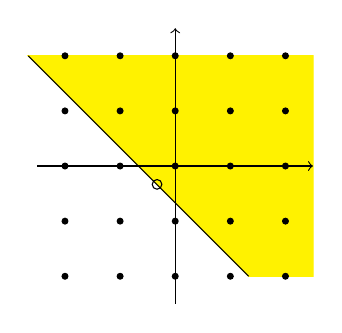
\begin{tikzpicture}[scale=0.7]
	
	\filldraw[yellow] (1.333,-2) -- (-2.667,2) -- (2.5,2) -- (2.5,-2) -- cycle;
	
	\foreach \x in {-2,...,2}
	\foreach \y in {-2,...,2}
	{
		\filldraw[fill=black] (\x,\y) circle (1.5pt);
	}
	\draw[->] (-2.5,0) -- (2.5,0);
	\draw[->] (0,-2.5) -- (0,2.5);
	\draw (1.333,-2) -- (-2.667,2);
	\draw (-0.33,-0.333) circle (2.5pt);
	\end{tikzpicture}
\end{center}

It is clear that the ``vertex'' is not a vertex in the strict sense, but only gives a displacement of the cone. The output when run in default mode:

\begin{Verbatim}
1 module generators
1 Hilbert basis elements of recession monoid
1 vertices of polyhedron
1 extreme rays of recession cone
2 support hyperplanes of polyhedron (homogenized)

embedding dimension = 3
affine dimension of the polyhedron = 2 (maximal)
rank of recession monoid = 2
internal index = 3
dimension of maximal subspace = 1

size of triangulation   = 1
resulting sum of |det|s = 3

dehomogenization:
0 0 1 


module rank = 1

***********************************************************************

1 module generators:
0 0 1

1 Hilbert basis elements of recession monoid:
0 1 0

1 vertices of polyhedron:
0 -2 3

1 extreme rays of recession cone:
0 1 0

1 basis elements of maximal subspace:
1 -1 0

2 support hyperplanes of polyhedron (homogenized):
0 0 1
3 3 2
\end{Verbatim}

The ``vertex'' of the polyhedron shown is of course the lifted version of the vertex modulo the maximal subspace. It is not the input ``vertex'', but agrees with it up to a unit.

\subsubsection{Checking pointedness first}\label{IsPointed}

Nonpointed cones will be an exception in Normaliz computations, and therefore Normaliz assumes that the (recession) cone it must compute is pointed. Only in rare circumstances it could be advisable to have this property checked first. There is no need to do so when the dual algorithm is used since it does not require the cone to be pointed. Moreover, if an explicit grading is given or a grading dependent computation is asked for, one cannot save time by checking the pointedness first.

The exceptional case is a computation, say of a Hilbert basis, by the primal algorithm in which the computation of the support hyperplanes needs very long time to be completed. If you are afraid this may happen, you can force Normaliz to compute the support hyperplanes right away by adding \verb|IsPointed| to the computation goals. This is a disadvantage only if the cone is unexpectedly pointed.

\subsubsection{Input of a subspace}\label{subspace}

If a linear subspace contained in the cone is known a priori, it can be given to Normaliz via the input type \verb|subspace|. If Normaliz detects a \verb|subspace|, it appends the rows of the matrix to the generators of the cone, and additionally the negative of the sum of the rows (since we must add the subspace as a cone). If \verb|subspace| is combined with \verb|cone_and_lattice|, then the rows of \verb|subspace| are also appended to the generators of the lattice. It is not assumed that the vectors in \verb|subspace| are linearly independent or generate the maximal linear subspace of the cone. A simple example (\verb|subspace4.in|):
\begin{Verbatim}
amb_space 4
cone 4
1 0 2 0
0 1 -2 1
0 0 0 1
0 0 0 -1
subspace 1
0 0 1 0
\end{Verbatim}

From the output:
\begin{Verbatim}
2 lattice points in polytope (Hilbert basis elements of degree 1):
 0 1 0 0
 1 0 0 0

0 further Hilbert basis elements of higher degree:

2 extreme rays:
 0 1 0 0
 1 0 0 0

2 basis elements of maximal subspace:
 0 0 1 0
 0 0 0 1

2 support hyperplanes:
 0 1 0 0
 1 0 0 0
\end{Verbatim}

One should note that the maximal subspace is generated by the smallest face that contains all invertible elements. Therefore, in order to make all vectors in a face invertible, it is enough to put a single vector from the interior of the face into \verb|subspace|.

\subsubsection{Data relative to the original monoid}

If original monoid generators are defined, there are two data related to them that must be read with care.

First of all, we consider the original monoid generators as being built from the vectors in \verb|cone| or \verb|cone_and_lattice| plus the vectors in \verb|subspace| and additionally the negative of the sum of the latter (as pointed out above).

The test for ``Original monoid is integrally closed'' is correct -- it returns \verb|true| if and only if the original monoid as just defined indeed equals the computed integral closure. (There was a mistake in version~3.0.)

The ``module generators over the original monoid'' only refer to the \emph{image} of the original monoid and the image of the integral closure \emph{modulo the maximal subspace}. They do not take into account that the unit group of the integral closure may not be generated by the original generators. An example in which the lack of integral closedness is located in the unit group (\verb|normface.in|):

\begin{Verbatim}
amb_space 5
cone 4
0 0 0 1 1
1 0 0 1 1
0 1 0 1 1
0 0 1 1 1
subspace 4
0 0 0 0 1
1 0 0 0 1
0 1 0 0 1
1 1 2 0 1
\end{Verbatim}

From the output file:

\begin{Verbatim}
...
dimension of maximal subspace = 4
original monoid is not integrally closed  in chosen lattice
unit group index = 2
...

1 lattice points in polytope (Hilbert basis elements of degree 1):
0 0 0 1 0
...
1 module generators over original monoid:
0 0 0 0 0
\end{Verbatim}
The original monoid is not integrally closed since the unit group of the integral closure is strictly larger than that of the original monoid: the extension has index $2$, as indicated. The quotients modulo the unit groups are equal, as can be seen from the generator over the original monoid or the Hilbert basis (of the integral closure) that is contained in the original monoid.


\subsection{Exporting the triangulation}\label{Triang}

The primal algorithm of Normaliz is based on ``triangulations''. What we call a ``triangulation'' here, is often only a collection of simplicial cones with properties that come close to those of a triangulation in the strict sense. Without being asked explicitly, Normaliz does not try to store and export its computational tool. In the file \verb|<project>.out| you can sometimes see words ``partial'' and ``nested''. ``Partial'' means that only a subset of the cone has been triangulated, and ``nested'' is explained below.
But if the user wants Normaliz to export a triangulation, then a triangulation in the strict sense is computed.

The option \ttt{Triangulation}, \ttt{-T} asks Normaliz to export a triangulation by writing the files
\ttt{<project>.tgn} and \verb|<project>.tri|:

\begin{itemize}
	
	\itemtt[tgn] The file \ttt{tgn} contains a matrix of vectors (in the
	coordinates of $\AA$) spanning the simplicial cones in
	the triangulation.
	
	\itemtt[tri]
	The file \ttt{tri} lists the simplicial subcones. There are two variants, depending on whether \verb|ConeDecomposition| had been set. Here we assume that \verb|ConeDecomposition| is not computed. See Section~\ref{Disjoint} for the variant with \verb|ConeDecomposition|.
	
	The first line contains the number of simplicial cones
	in the triangulation, and the next line contains the
	number $m+1$ where $m=\rank \EE$. Each of the following
	lines specifies a simplicial cone $\Delta$: the first
	$m$ numbers are the indices (with respect to the order
	in the file \ttt{tgn}) of those generators that span
	$\Delta$, and the last entry is the multiplicity of
	$\Delta$ in $\EE$, i.e., the absolute value of the
	determinant of the matrix of the spanning vectors (as
	elements of $\EE$).
\end{itemize}

The following example is the $2$-dimensional cross polytope with one excluded face (\verb|cross2.in|). The excluded face is irrelevant for the triangulation.

\begin{Verbatim}
amb_space 3
polytope 4
1 0
0 1
-1 0
0 -1
excluded_faces 1
-1 -1 1
Triangulation
StanleyDec        
\end{Verbatim}
(The Stanley decomposition will be discussed in Section~\ref{Stanley}.)
Its \verb|tgn| and \verb|tri| files are
\begin{Verbatim}
tgn         tri
4           2
3           4
-1 0 1      1 2 3    2
0 -1 1      2 3 4    2
0 1 1       
1 0 1 
\end{Verbatim}

We see the $4$ vertices $v_1,\dots,v_4$ in homogenized coordinates in \verb|tgn| and the $2$ simplices (or the simplicial cones over them) in \verb|tri|: both have multiplicity $2$.


In addition to the files \verb|<project>.tgn| and \verb|<project>.tri|, also the file \verb|<object>.inv| is written. It contains the data of the file \verb|<project>.out| above the line of stars in a human and machine readable format.

\textbf{Note:}\enspace Normaliz (now) allows the computation of triangulations for all input. In the homogeneous case it computes a triangulation of the (pointed quotient of the) cone $C$ defined by the input. It can then be interpreted as a triangulation of a cross-section polytope if a grading is given. In the inhomogeneous case for which the input defines a polyhedron $P$, $C$ is the cone over $P$. If $P$ is a polytope, then a triangulation of $C$ can again be identified with a triangulation of $P$. However, if $P$ is unbounded, the the triangulation of $C$ only induces a polyhedral decomposition of $P$ into subpolyhedra whose compact faces are simplices.

\subsubsection{Nested triangulations}\label{nested}
We explain what we mean by a nested triangulation, even if it cannot be exported.
If Normaliz has subdivided a simplicial cone of a triangulation of the cone $C$, the resulting decomposition of $C$ may no longer be a triangulation in the strict sense. It is rather a \emph{nested triangulation}, namely a map from a rooted tree to the set of full-dimensional subcones of $C$ with the following properties:
\begin{arab}
	\item the root is mapped to $C$,
	\item every other node is mapped to a full dimensional simplicial subcone,
	\item the simplicial subcones corresponding to the branches at a node $x$ form a triangulation of the simplicial cone corresponding to $x$.
\end{arab}

The following figure shows a nested triangulation:

\begin{center}
	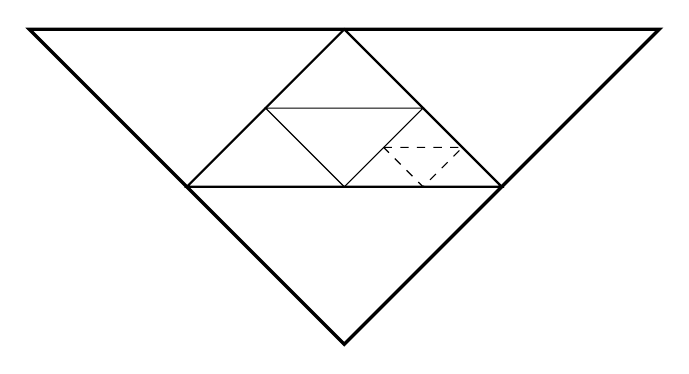
\begin{tikzpicture}[scale=1.0]
	\draw[very thick] (-4,4) -- (4,4) -- (0,0) -- cycle;
	\draw[thick] (-2,2) -- (2,2) -- (0,4) -- cycle;
	\draw (-1,3) -- (1,3) -- (0,2) -- cycle;
	\draw[dashed] (0.5,2.5) --(1.5,2.5) -- (1.0,2) --cycle;
	\end{tikzpicture}
\end{center}

For the Normaliz computations, nested triangulations are as good as ordinary triangulations, but in other applications the difference may matter. With the option \verb|-T|, Normaliz prints the leaves of the nested triangulation to the \verb|tri| file. They constitute the simplicial cones that are finally evaluated by Normaliz. The subdivision can be blocked by \verb|NoSubdivision|, independently of the computation goals.

The triangulation is always plain if \verb|-T| is used, or if one of the refined triangulations below is computed.

\subsubsection{Disjoint decomposition}\label{Disjoint}

Normaliz can export the disjoint decomposition of the cone that it has computed. This decomposition is always computed together with a full triangulation, unless only the multiplicity is asked for. It represents the cone as the disjoint union of semiopen simplicial subcones. The corresponding closed cones constitute the triangulation, and from each of them some facets are removed so that one obtains a disjoint decomposition. In the following figure, the facets separating the triangles are omitted in the triangle on the $-$ side.

\begin{center}
	\begin{scriptsize}
		%\tikzstyle{every node}=[circle, draw, fill=black, inner sep=0pt, minimum width=3pt]
		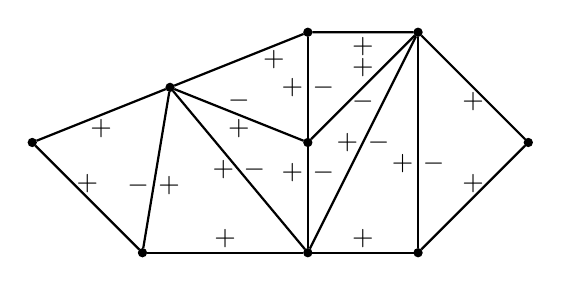
\begin{tikzpicture}
		[scale=0.7,auto=left, thick]
		%\foreach \from/\to in {n2/n4,n2/n5,n4/n5,n4/n6,n5/n7,n6/n7}
		%  \foreach \x in {0, 1, ..., 9}
		\foreach \x/\y in {0/2, 2/0, 5/0, 5/2, 5/4, 7/0, 7/4, 9/2}
		\node [circle, draw, fill=black, inner sep=0pt, minimum width=2.5pt](n\x\y) at (\x,\y) {};
		\node [circle, draw, fill=black, inner sep=0pt, minimum width=2.5pt](n23) at (2.5,3) {};
		%\node [circle, draw, inner sep=0pt, minimum width=3pt, label=above:$O_C$](OC) at (2.8,1.7) {};
		
		%  \draw (\from) -- node[above]{$+$} node[below]{$-$} (\to);
		\draw (n20) -- node[right=-2pt, pos=0.4]{$+$} node[left=-2pt, pos=0.4]{$-$} (n23);
		\draw (n20) -- node[above=-2pt]{$+$} (n02);
		\draw (n50) -- node[right=-2pt]{$-$} node[left=-2pt]{$+$} (n23);
		\draw (n50) -- node[near end, right=-2pt]{$-$} node[near end, left=-2pt]{$+$} (n52);
		\draw (n52) -- node[right=-2pt]{$-$} node[left=-2pt]{$+$} (n54);
		\draw (n70) -- node[right=-2pt, pos=0.4]{$-$} node[left=-2pt, pos=0.4]{$+$} (n74);
		
		\draw (n52) -- node[below=-2pt]{$+$} node[above=-2pt]{$-$} (n23);
		\draw (n52) -- node[below=-2pt]{$-$} node[above]{$+$} (n74);
		\draw (n50) -- node[right=-2pt]{$-$} node[left=-2pt]{$+$} (n74);
		
		\draw (n02) -- node[below=-2pt]{$+$} (n23);
		\draw (n23) -- node[right=5pt]{$+$} (n54);
		\draw (n20) -- node[above=-2pt]{$+$} (n50);
		\draw (n50) -- node[above=-2pt]{$+$} (n70);
		\draw (n54) -- node[below=-2pt]{$+$} (n74);
		\draw (n70) -- node[above=-2pt]{$+$} (n92);
		\draw (n74) -- node[below=-2pt]{$+$} (n92);	
		
		%  \draw[to] (daq) -- node[midway,right] {raw event data\\level 1} (buffer);
		% \draw[to] (monitor) -- node[midway,above] {events} node[midway,below] {level 1} (datastore);
		\end{tikzpicture}
	\end{scriptsize}
\end{center}

If you want to access the disjoint decomposition, you must activate the computation goal \verb|ConeDecomposition| or use the command line option is \verb|-D|. As an example we compute \verb|cross2.in| with the computation goal \verb|ConeDecomposition|. The file \verb|cross2.tri| now looks as follows:

\begin{Verbatim}
2
7
1 2 3    2    0 0 0
2 3 4    2    0 0 1
\end{Verbatim}

As before the first line contains the size of the triangulation and the second is the number of entries of each row.
The first $3$ entries in each line are the indices of the extreme rays with respect to the \verb|tgn| file and the fourth entry is the determinant. They are followed by a $0/1$ vector indicating the open facets in the order in which they are opposite to the extreme rays. If the corresponding entry is $1$, the facet must be removed.

In our example all facets of the first simplicial cone are kept, and from the second simplicial cone the facet opposite to the third extreme ray (with index $4$ relative to \verb|tgn|) must be removed.

The disjoint decomposition which is the basis of all Hilbert series computations uses the algorithm suggested by K\"oppe and Verdoolaege~\cite{KV}.

\subsection{Terrific triangulations}

The basic triangulation computed by the Normaliz primal algorithm is a collection of simplicial cones each of which is generated by a subset of the generators of the cone $C$ that is computed. Neither it is guaranteed that every generator of $C$ appears as a generator of one of the simplicial cones, nor that every lattice point of a polytope participates in the triangulation. Moreover, there is no restriction on the determinants of the simplicial cones. Normaliz offers refined triangulations that satisfy the type of condition just mentioned. The refined triangulations start from the basic triangulation and refine it by iterated stellar subdivision. For background information we recommend~\cite{BG}, especially Chapter~2.

All these triangulations are ``plain'' and ``full''. Moreover, Normaliz can hold only a single triangulation. Therefore the refined triangulations exclude each other mutually.

The number of simplicial cones and the determinant sum appearing in the output file refer to the basic triangulation. The files \ttt{tri} and {tgn} contain the refined triangulation. It is not possible to derive a disjoint cone decomposition from a refined triangulation.

\emph{Warning.}\enspace Refined triangulations can become very large. For example, for \ttt{small.in} the basic triangulation has $4580$ simplicial cones, but the \verb|LattcicePointTriangulation| has $739,303$ of them. For the unimodular triangulation the number rises to $49,713,917$, and the number of rays is $5,558,042$, whereas the number of lattice points is only $34,591$. You should use \verb|LongLong| whenever possible.

In addition to the refined triangulations Normaliz offers \emph{placing} and \emph{pulling} triangulations which are defined combinatorially with respect to the order in which the generators are inserted.

\subsubsection{Just Triangulation}
Our running example in the following is \ttt{square2.in} :
\begin{Verbatim}
amb_space 3
cone 6
0 0 1
0 2 1
2 0 1
2 1 1
2 2 1
3 3 2
Triangulation
/* AllGeneratorsTriangulation */
/* LatticePointTriangulation */
/* UnimodularTriangulation */
/* PullingTriangulation */
\end{Verbatim}
The input file defines a square in the plane. For demonstration purposes we have added two generators to the first four that define the vertices of the square. The output is the basic triangulation:

\begin{minipage}{0.6\textwidth}
\begin{Verbatim}
tri                tgn
3                  6
4                  3
1 2 3    4         0 0 1 
2 3 4    2         0 2 1 
2 4 5    2         2 0 1 
                   2 1 1 
                   2 2 1 
                   3 3 2 
\end{Verbatim}
\end{minipage}
\begin{minipage}{0.4\textwidth}
	\begin{center}
		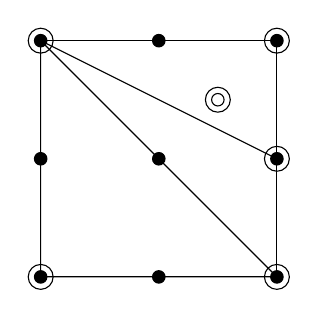
\begin{tikzpicture}[scale=1.5]
		\foreach \x in {0,...,2}
		\foreach \y in {0,...,2}
		{
			\filldraw[fill=black] (\x,\y) circle (1.5pt);
		}
		\draw (0,0) -- (2,0) -- (2,2) -- (0, 2) -- cycle;
		\draw (0,0) -- (2,0) -- (0, 2) -- cycle;
		\draw (2,1) -- (0,2);
		\draw (0,0) circle(3pt);
		\draw (2,0) circle(3pt);
		\draw (0,2) circle(3pt);
		\draw (2,2) circle(3pt);
		\draw (2,1) circle(3pt);
		\draw (1.5,1.5) circle(3pt);
		\draw (1.5,1.5) circle (1.5pt);
		\end{tikzpicture}
	\end{center}
\end{minipage}

Normaliz sorts the generators lexicographically by default so that $(2,1,1)$ is inserted into cone building before $(2,2,1)$. If you add \ttt{KeepOrder} to the input, the basic triangulation will have only $2$ triangles: the square is subdivided along its diagonal.

\textbf{Note:}\enspace The remark in Section~\ref{Triang} about the interpretation of general triangulations applies to the refined triangulations as well. The refined triangulations are computed for the cone over the polyhedron if the input is inhomogeneous. \ttt{LatticePointTriangulation} is only allowed if the input defines a polytope.

\subsubsection{All generators triangulation}
The option
\begin{itemize}
	\itemtt[AllGeneratorsTriangulation]
\end{itemize}
asks for a triangulation such that all generators appear as rays in it. (It can be added to \ttt{Triangulation}, but can also be used alone.) For our example we get

\begin{minipage}{0.6\textwidth}
\begin{Verbatim}
tri                tgn
5                  6
4                  3
1 2 3    4         0 0 1 
2 3 4    2         0 2 1 
4 5 6    1         2 0 1 
2 5 6    2         2 1 1 
2 4 6    1         2 2 1 
                   3 3 2 
\end{Verbatim}
\end{minipage}
\begin{minipage}{0.4\textwidth}
	\begin{center}
		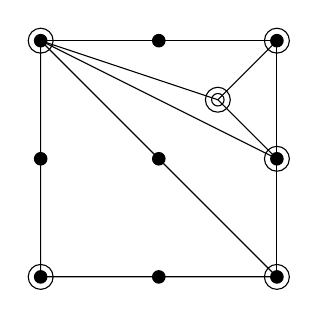
\begin{tikzpicture}[scale=1.5]
		\foreach \x in {0,...,2}
		\foreach \y in {0,...,2}
		{
			\filldraw[fill=black] (\x,\y) circle (1.5pt);
		}
		\draw (0,0) -- (2,0) -- (2,2) -- (0, 2) -- cycle;
		\draw (0,0) -- (2,0) -- (0, 2) -- cycle;
		\draw (2,1) -- (0,2);
		\draw (0,0) circle(3pt);
		\draw (2,0) circle(3pt);
		\draw (0,2) circle(3pt);
		\draw (2,2) circle(3pt);
		\draw (2,1) circle(3pt);
		\draw (1.5,1.5) circle(3pt);
		\draw (1.5,1.5) circle (1.5pt);
		\draw (1.5,1.5) -- (2,2);
		\draw (1.5,1.5) -- (2,1);
		\draw (1.5,1.5) -- (0,2);
		\end{tikzpicture}
	\end{center}
\end{minipage}

\subsubsection{Lattice point triangulation}

The option
\begin{itemize}
	\itemtt[LatticePointTriangulation]
\end{itemize}
asks for a triangulation such that all lattice points of a polytope appear as vertices in it. (It can be added to \ttt{Triangulation}, but can also be used alone.) This option implies \ttt{LatticePoints} and, therefore, \ttt{NoGradingDenom}. For our example we get


\begin{minipage}{0.6\textwidth}
\begin{Verbatim}
tri               tgn
8                 10
4                 3
3 4 9    1        0 0 1
2 4 9    1        0 2 1
4 5 10    1       2 0 1
2 4 10    1       2 1 1
3 7 8    1        2 2 1
1 7 8    1        3 3 2
3 7 9    1        0 1 1
2 7 9    1        1 0 1
                  1 2 1
\end{Verbatim}
\end{minipage}
\begin{minipage}{0.4\textwidth}
	\begin{center}
		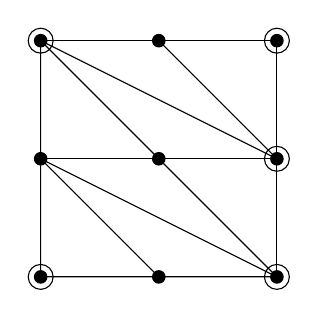
\begin{tikzpicture}[scale=1.5]
		\foreach \x in {0,...,2}
		\foreach \y in {0,...,2}
		{
			\filldraw[fill=black] (\x,\y) circle (1.5pt);
		}
		\draw (0,0) -- (2,0) -- (2,2) -- (0, 2) -- cycle;
		\draw (0,0) -- (2,0) -- (0, 2) -- cycle;
		\draw (2,1) -- (0,2);
		\draw (0,0) circle(3pt);
		\draw (2,0) circle(3pt);
		\draw (0,2) circle(3pt);
		\draw (2,2) circle(3pt);
		\draw (2,1) circle(3pt);
		\draw (0,1) -- (2,1);
		\draw (1,2) -- (2,1);
		\draw (1,0) -- (0,1);
		\draw (0,1) -- (2,0);
		\end{tikzpicture}
	\end{center}
\end{minipage}

\subsubsection{Unimodular triangulation}

The option
\begin{itemize}
	\itemtt[UnimodularTriangulation]
\end{itemize}
asks for a triangulation such that all generators appear as rays in it. (It can be added to \ttt{Triangulation}, but can also be used alone.) The goal is a triangulation into simplicial cones of determinant $1$. It implies \ttt{HilbertBasis} since all elements of the Hilbert basis must appear as rays in a unimodular triangulation, but in general further vectors must be used.

\ttt{UnimodularTriangulation} is not allowed in inhomogeneous computations or for algebraic polyhedra.

For our example above we get nothing new since lattice point triangulations of $2$-dimensional lattice polytopes are automatically unimodular. We recommend to run \ttt{polytope.in} with the option \ttt{UnimodularTriangulation}.

\subsubsection{Placing triangulation}\label{PlacingTri}

This is very close to the basic triangulation that Normaliz computes, except that for the basic triangulation Normaliz takes the freedom to reorder the generators and to apply bottom decomnposition if it seems to be useful If you insist on
\begin{itemize}
	\itemtt[PlacingTriangulation]
\end{itemize}
then these manipulations are excluded. The generators are inserted exactly in the order as Normaliz gets them. The triangulation is built incrementally: if the polytope (or cone) $P$ is extended by the next generator $x$ to form the polytope $Q$, then the triangulation is augmented by all simplices that arise as the convex (or conical) hulls of the new generators and the faces of the `òld'' triangulation that are in those facets of $P$ which are \emph{visible} from $x$. In particular this means that the new triangulation of $Q$ is exactly the old of $P$ if $x\in P$.

For our running example \verb|PlacingTiangulations| gives the same result as \verb|Triangulation|, and therefore we don't repeat the output.

Placing triangulations arise as \emph{lexicographic} triangulations in the context of Gröbner bases of toric ideals; see Sturmfels \cite[p. 67]{Stu}.

\subsubsection{Pulling triangulation}\label{PullingTri}

For the pulling triangulation,
\begin{itemize}
	\itemtt[PullingTriangulation]
\end{itemize}
the generators are also inserted in the order given. However, the extension from $P$ to $Q$ follows are different rule: now the new triangulation is formed by taking the convex (or conical) hull of the new generator $x$ and all  faces of the `òld'' triangulation that are in those facets of $P$ which are \emph{invisible} from $x$ and their collection replaces theòld triangulation -- it is indeed a triangulation of $Q$. If $x\in P$, then the invisible facets of $P$ are those that do not contain $x$. One consequence is that the last inserted generator is in all facets of the pulling triangulation. 

For our running example we get

\begin{minipage}{0.6\textwidth}
	\begin{Verbatim}
tri              tgn
4                6
4                3
1 2 6    6       0 0 1 
1 3 6    6       0 2 1 
2 5 6    2       2 0 1 
3 5 6    2       2 1 1 
                 2 2 1 
                 3 3 2 
	\end{Verbatim}
\end{minipage}
\begin{minipage}{0.4\textwidth}
	\begin{center}
		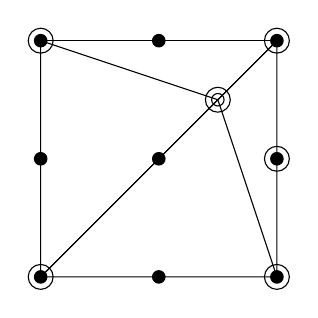
\begin{tikzpicture}[scale=1.5]
		\foreach \x in {0,...,2}
		\foreach \y in {0,...,2}
		{
			\filldraw[fill=black] (\x,\y) circle (1.5pt);
		}
		\draw (0,0) -- (2,0) -- (1.5,1.5) -- (0, 0) -- cycle;
		\draw (0,0) -- (0,2) -- (1.5,1.5) -- (2,2) -- cycle;
		\draw (2,0) -- (2,2) -- (1.5,1.5);
		\draw (0,2) -- (2,2);
		\draw (0,0) circle(3pt);
		\draw (2,0) circle(3pt);
		\draw (0,2) circle(3pt);
		\draw (2,2) circle(3pt);
		\draw (2,1) circle(3pt);
		\draw (1.5,1.5) circle(3pt);
		\draw (1.5,1.5) circle (1.5pt);
		\end{tikzpicture}
	\end{center}
\end{minipage}

Pulling triangulations arise as \emph{reverse lexicographic} triangulations in the context of Gröbner bases of toric ideals; see Sturmfels \cite[p. 67]{Stu}.

\subsection{Exporting the Stanley decomposition}\label{Stanley}

The computation goal \ttt{StanleyDec}, \ttt{-y} makes Normaliz
write the files \ttt{<project>.tgn}, \verb|<project>.dec| and \verb|<project>.inv|. Stanley decomposition is contained in the file with the suffix \verb|dec|. But this file also contains the inclusion/exclusion data if there are excluded faces:

(a) If there are any excluded faces, the file starts with the word
\verb|in_ex_data|. The next line contains the number of such data that follow.
Each of these lines contains the data of a face and the coefficient with which
the face is to be counted: the first number lists the number of generators that
are contained in the face, followed by the indices of the generators relative
to the \verb|tgn| file and the last number is the coefficient.

(b) The second block (the first if there are no excluded faces) starts with
the word \verb|Stanley_dec|, followed by the number of simplicial cones in the
triangulation.

For each simplicial cone $\Delta$ in the
triangulation this file contains a block of data:
\begin{enumerate}
	\item[(i)] a line listing the indices $i_1,\dots,i_m$ of the
	generators $v_{i_1},\dots,v_{i_m}$ relative to the
	order in \ttt{tgn} (as in \ttt{tri}, $m=\rank \EE$);
	
	\item[(ii)] a $\mu\times m$ matrix where $\mu$ is the
	multiplicity of $\Delta$ (see above).
	
	In the notation of~\cite{BIS}, each line lists an
	``offset'' $x+\epsilon(x)$ by its coordinates with
	respect to $v_{i_1},\dots,v_{i_m}$ as follows: if
	$(a_1,\dots,a_m)$ is the line of the matrix, then
	$$
	x+\epsilon(x)=\frac{1}{\mu}(a_1v_{i_1}+\dots+a_mv_{i_m}).
	$$
\end{enumerate}


The \verb|dec| file of the example \verb|cross2.in| is
\begin{Verbatim}
in_ex_data
1
2 3 4 -1
Stanley_dec
2
1 2 3        2 3 4 
2            2
3            3
0 0 0        0 0 2 
0 1 1        1 1 2 
\end{Verbatim}
For reference: \verb|cross2.tgn| is
\begin{Verbatim}
4
3
-1 0 1 
0 -1 1 
0 1 1 
1 0 1 
\end{Verbatim}

There is $1$ face in \verb|in_ex_data| (namely the excluded one), it contains the $2$ generators $v_3$ and $v_4$ and appears with multiplicity $-1$. The Stanley decomposition consists of $4$ components of which each of the simplicial cone contains $2$. The second offset in the second simplicial cone is
$$
\frac12 (1v_2+1v_3+2v_4)=(1,0,2).
$$

Another input file in \verb|example| is \verb|Stanleydec.in|.

\textbf{Note:}\enspace The computation and export of the Stanley decomposition in the inhomogeneous case is the same as that of triangulations: it is computed for the cone over the polyhedron.

\subsection{Face lattice, f-vector and incidence matrix}\label{FaceLattice}

In connection with ``face'', ``lattice'' means a partially ordered set with meet and join. Every face of a polyhedron is the intersection of the facets that contain it, and therefore Normaliz computes all intersections of facets, including the polyhedron itself and the empty set if the intersection of all facets should be empty.

There are three relevant computation goals:
\begin{itemize}
	\itemtt[FaceLattice]
	\itemtt[FVector]
	\itemtt[Incidence]
\end{itemize}
The names are more or less self explanatory and discussed in the following.

The computation of the face lattice or just the f-vector might require very much memory. Therefore one should be careful if the dimension is large or there are many support hyperplanes.

The file \verb|rationalFL.in| contains
\begin{Verbatim}
amb_space 3
polytope 3
1/2 1/2
-1/3 -1/3
1/4 -1/2
HilbertSeries
FaceLattice
Incidence
\end{Verbatim}
representing a rational triangle. (Without \verb|FaceLattice| it has been discussed in Section~\ref{rational}.) (\verb|Incidence| is discussed below.
)

Since the face lattice can be very large, it is returned as a separate file \verb|<project>.fac|. For our example we get \verb|rationalFL.fac|:
\begin{Verbatim}
8
3

000 0
100 1
010 1
110 2
001 1
101 2
011 2
111 3
primal
\end{Verbatim}
The first line contains the number of faces, and the second the number of facets. The other lines list the faces $F$, encoded by a a $0$-$1$-vector and an integer. The integer is the codimension of $F$. The $0$-$1$-vector lists the facets containing $F$: the entry $1$ at the $i$-th coordinate indicates that the $i$-th facet contains $F$.

The attribute \verb|primal| indicates that we have computed the face lattice on the primal side. Dual face lattices will be introduced below.

The facets are counted as in the main output file \verb|<project>.out|. (If you want them in a separate file, activate the output file \verb|<project>.cst|.) In our case the support hyperplanes are:
\begin{Verbatim}
-8 2 3 
1 -1 0 
2 7 3
\end{Verbatim}
So, for example, the face \verb|011| is contained in the facets given by the linear forms $(1,-1,0)$ and
$(2,7,3)$: it is the vertex $(1/2,1/2,1)$ (in homogeneous coordinates). The first face \verb|000| is the intersection of the empty set of facets, namely the full triangle, and the last face \verb|111| is the empty set.

Note that one can set a bound on the codimension of the faces that are to be computed. See Section~\ref{codim_bound}.

One can retrieve the incidence matrix using the computation goal \verb|Incidence|. It is printed to the file \verb|<project>.inc|. The format of this files is illustrated by two examples. The first is \verb|rationalFL| again, with its homogeneous input:
\begin{Verbatim}
3
0
3

101
110
011
primal
\end{Verbatim}
The first line contains the number of support hyperplanes, the second the number of vertices of the polyhedron ($0$ for homogeneous input), and the third the number of extreme rays of the (recession) cone. The following lines list the incidence vectors of the facets. They are ordered in the same way as the support hyperplanes in the main output file. The incidence vector has entry $1$ for an extreme ray (or) vertex) contained in the facet, and $0$ otherwise. The extreme rays are ordered as in the main output file.

In the inhomogeneous case each line starts with the incidence for the vertices of the polyhedron, followed by the extreme rays of the recession cone. An example is \verb|InhomIneqInc.inc|
\begin{Verbatim}
3
2
1

01  1
10  1
11  0
primal
\end{Verbatim}
with its $2$ vertices and $1$ extreme ray of the recession cone.

\subsubsection{Dual face lattice, f-vector and incidence matrix}

Normaliz can also compute the face lattice of the dual cone.  The relevant computation goals:
\begin{itemize}
	\itemtt[DualFaceLattice]
	\itemtt[Dual[FVector]
	\itemtt[DualIncidence]
\end{itemize}

On the primal side this means that the face lattice is built bottom up and each face is represented by the extreme rays it contains. Since this is not possible for unbounded polyhedra, the dual versions are restricted to homogeneous input or inhomogeneous input defining polytopes. One application of the dual version is the computation of faces of low dimension which may be difficult to reach from the top if there are many facets. The numerical \verb|face_codim_bound| now refers to the face codimension on the dual side. For example, if one wants to compute the edges of a polytope from the vertices, \verb|face_codim_bound| must be set to $2$ since the edges define codimension $2$ faces of the dual polytope.

An example (\verb|cube_3_dual_fac.in|):
\begin{Verbatim}
amb_space 3
constraints 6 symbolic
x[1] >= 0;
x[2] >= 0;
x[3] >= 0;
x[1] <= 1;
x[2] <= 1;
x[3] <= 1;
DualFaceLattice
DualIncidence
face_codim_bound 2
\end{Verbatim}

In the output file we see
\begin{Verbatim}
dual f-vector (possibly truncated):
12 8 1
\end{Verbatim}
which is the f-vector of the dual polytope (or cone) starting from codimension $2$ and going up to codimension $0$.

The dual face lattice up to codimension $2$ is given by is given by
\begin{Verbatim}
21
8

00000000 0
10000000 1
...
00000011 2
dual
\end{Verbatim}
Indeed, we have $21$ faces in that range, and each face is specified by the vertices (or extreme rays) it contains. The attribute \verb|dual| helps to recognize the dual situation.

The dual incidence matrix lists the support hyperplanes containing the vertices (or extreme rays):
\begin{Verbatim}
8
0
6

000111
...
111000
dual
\end{Verbatim}
For the cube defined by inhomogeneous input we have $8$ vertices of the polyhedron, $0$ extreme rays of the recession cone and $6$ facets.

Primal and dual versions of face lattice and incidence, respectively, are printed to the same file. Therefore only one of them is allowed.

\subsubsection{Only up to orbits}

There are computation goals that allow to compute (only) the orbits of faces and f-vectors counting the orbits in each dimension:
\begin{itemize}
	\itemtt[FaceLatticeOrbits]
	\itemtt[FVectorOrbits]
	\itemtt[DualFaceLatticeOrbits]
	\itemtt[DualFVectorOrbits]
\end{itemize}

These computation goals require an automorphism group. Since there are several reasonable choices, Normaliz does not btry to guess a type. Note that these are not pure output options. Depending on the size of the automorphism group they may help to extend the range of face lattice computations. Example: \verb*|SubModularConeN4.in|.

In later versions these computation goals may be renamed.

\subsection{Module generators over the original monoid}\label{MinMod}

Suppose that the original generators are well defined in the input. This is always the case when these consists just of a \verb|cone| or a \verb|cone_and_lattice|. Let $M$ be the monoid generated by them. Then Normaliz computes the integral closure $N$ of $M$ in the effective lattice $\EE$. It is often interesting to understand the difference set $N\setminus M$. After the introduction of a field $K$ of coefficients, this amounts to understanding $K[N]$ as a $K[M]$-module. With the option \verb|ModuleGeneratorsOverOriginalMonoid, -M| Normaliz computes a minimal generating set $T$ of this module. Combinatorially this means that we find an irreducible cover
$$
N=\bigcup_{x\in T} x+M.
$$
Note that $0\in T$ since $M\subset N$.
\begin{center}
	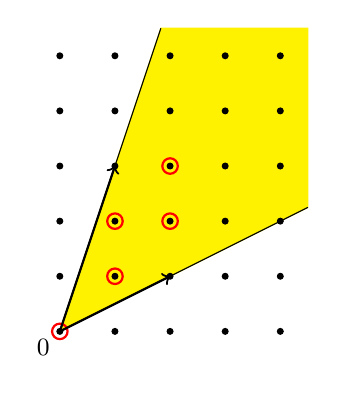
\begin{tikzpicture}[scale=0.7]
	\filldraw[yellow] (0,0) -- (1.833,5.5) -- (4.5,5.5) -- (4.5,2.25) -- cycle;
	\draw (0,0) -- (1.833,5.5);
	\draw (0,0) -- (4.5,2.25) node at (-0.3,-0.3){\small $0$};
	\foreach \x in {0,...,4}
	\foreach \y in {0,...,5}
	{
		\filldraw[fill=black] (\x,\y) circle (1.5pt);
	}
	\draw[red,thick] (1,1) circle (4pt);
	\draw[red,thick] (2,3) circle (4pt);
	\draw[red,thick] (1,2) circle (4pt);
	\draw[red,thick] (2,2) circle (4pt);
	\draw[red,thick] (0,0) circle (4pt);
	\draw[->,thick] (0,0) -- (1,3);
	\draw[->,thick] (0,0) -- (2,1);
	\end{tikzpicture}
\end{center}
As an example, we can run \verb|2cone.in| with the option \verb|-M| on the command line. This yields the output
\begin{Verbatim}
...
4 Hilbert basis elements:                                      
1 1                                                           
1 2                  5 module generators over original monoid:
1 3                   0 0                                     
2 1                   1 1                                     
                      1 2                                     
2 extreme rays:       2 2                                     
1 3                   2 3                                     
2 1                                                           
\end{Verbatim}

In the nonpointed case Normaliz can only compute the module generators of $N/N_0$ over $M/(M\cap N_0)$ where $N_0$ is the unit group of $N$. If $M_0\neq M_0$, this is not a system of generators of $M$ over $N$.

\subsubsection{An inhomogeneous example}

Let us have a look at a very simple input file (\verb|genmod_inhom2.in|):
\begin{Verbatim}
amb_space 2
cone 2
0 3
2 0
vertices 1
0 0 1
ModuleGeneratorsOverOriginalMonoid
\end{Verbatim}

The cone is the positive orthant that we have turned into a polyhedron by adding the vertex $(0,0)$. The original monoid is generated by $(2,0)$ and $(0,3)$.

In addition to the original monoid $M$ and its integral closure $N$ we have a third object, namely the module $P$ of lattice points in the polyhedron.We compute
\begin{enumerate}
	\item the system of generators of $P$ over $N$ (the \verb|module generators|) and
	\item the system of generators of $P$ over $N$ (the \verb|module generators over original monoid|).
\end{enumerate}
We do not compute the system of generators of $N$ over $M$ (that we get in the homogeneous case).

The output:
\begin{Verbatim}
1 module generators
2 Hilbert basis elements of recession monoid
1 vertices of polyhedron
2 extreme rays of recession cone
6 module generators over original monoid
3 support hyperplanes of polyhedron (homogenized)

embedding dimension = 3
affine dimension of the polyhedron = 2 (maximal)
rank of recession monoid = 2
internal index = 6

size of triangulation   = 1
resulting sum of |det|s = 6

dehomogenization:
0 0 1 


module rank = 1

***********************************************************************

1 module generators:
 0 0 1

2 Hilbert basis elements of recession monoid:
 0 1 0
 1 0 0

1 vertices of polyhedron:
 0 0 1

2 extreme rays of recession cone:
 0 1 0
 1 0 0

6 module generators over original monoid:
 0 0 1
 0 1 1
 0 2 1
 1 0 1
 1 1 1
 1 2 1

3 support hyperplanes of polyhedron (homogenized):
 0 0 1
 0 1 0
 1 0 0
\end{Verbatim}

\subsection{Lattice points in the fundamental parallelepiped}\label{LattPointsFPE}

Let $u_1,\dots,u_n$ be linearly independent vectors in $\ZZ^d\subset\RR^d$. They span a simplicial cone $C$. Moreover let $U$ be the subgroup of $(\RR^d,+)$ generated by $u_1,\dots,u_n$ and let $v\in\RR^d$. We are interested in the shifted cone $C'=v+C$. We assume that $C'$ contains a lattice point. This need not be true if $n<s$, but with our assumption we can also assume that $n=d$ after the restriction to the affine space spanned by $C'$. The \emph{fundamental} parallelepiped of $C$ (with respect to $U$) is
$$
F=\para(u_1,\dots,u_d)=\{q_qu_1+\dots+q_du_d: 0\le q_i<1\}.
$$
Set $F'=v+F$. Then the translates $u+F'$, $u\in U$, tile $\RR^d$; so $F'$ is a fundamental domain for the action of $U$ on $\RR^d$ by translation, and we call it $F'$ the \emph{fundamental} parallelepiped of $C'$ (with respect to $U$). Every point in $\RR^d$ differs from exactly one point in $F'$ by an element of $U$. This holds in particular for the lattice points.

One of the main basic tasks if Normaliz is the computation of the lattice points in $F'$, especially in the case $v=0$ (but not only). Looking back at the examples in Section~\ref{MinMod}, we see that we can in fact compute and export these lattice points via the computation goal \verb|ModuleGeneratorsOverOriginalMonoid|.

Often however, an additional complication comes up: we must shift $F'$ by an infinitesimally small vector in order to exclude certain facets of $C'$. This would be difficult in Normaliz without the input type \verb|open_facets| (see Section~\ref{open_facets}). Recall that this is a $0$-$1$-vector whose entries $1$ indicate which facets must be avoided: if its $i$-th entry is $1$, then the facet opposite to $v+u_i$ must be made ``open''.

The input file \verb|no_open_facets.in| is
\begin{Verbatim}
amb_space 2
cone 2
1 1
-3 3
vertices 1
1/2 1/2 1
ModuleGeneratorsOverOriginalMonoid
\end{Verbatim}

Then \verb|no_open_facets.out| contains
\begin{Verbatim}
6 module generators over original monoid:
-2 3 1
-1 2 1
-1 3 1
 0 1 1
 0 2 1
 1 1 1
\end{Verbatim}
These are $6$ encircled points in the left figure.

\begin{center}
	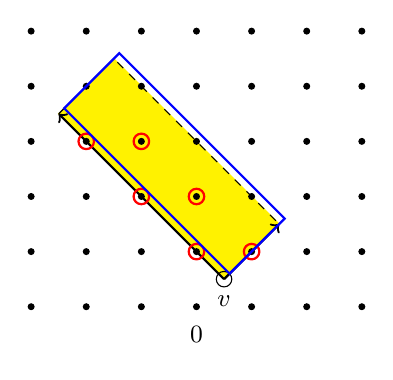
\begin{tikzpicture}[scale=0.7]
	\filldraw[yellow] (0.5,0.5) -- (1.5,1.5) -- (-1.5,4.5) -- (-2.5,3.5) -- cycle;
	\foreach \x in {-3,...,3}
	\foreach \y in {0,...,5}
	{
		\filldraw[fill=black] (\x,\y) circle (1.5pt);
	}
	\draw[->,thick] (0.5,0.5) -- (-2.5,3.5);
	\draw[->,thick] (0.5,0.5) -- (1.5,1.5);
	\draw[dashed] (-2.5,3.5) -- (-1.5,4.5) -- (1.5,1.5);
	\draw node at (0,-0.5){\small $0$};
	\draw node at (0.5,0.1){\small $v$};
	\draw[red,thick] (1,1) circle (4pt);
	\draw[red,thick] (0,1) circle (4pt);
	\draw[red,thick] (-1,2) circle (4pt);
	\draw[red,thick] (0,2) circle (4pt);
	\draw[red,thick] (-2,3) circle (4pt);
	\draw[red,thick] (-1,3) circle (4pt);
	\draw (0.5,0.5) circle (4pt);
	\draw[blue, thick] (0.6,0.6) -- (1.6,1.6) -- (-1.4,4.6) -- (-2.4,3.6) -- cycle;
	\end{tikzpicture}
	\qquad\qquad\qquad
	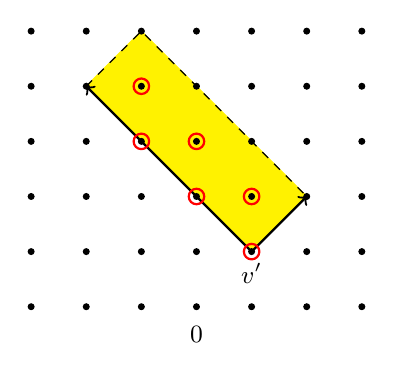
\begin{tikzpicture}[scale=0.7]
	\filldraw[yellow] (1,1) -- (2,2) -- (-1,5) -- (-2,4) -- cycle;
	\foreach \x in {-3,...,3}
	\foreach \y in {0,...,5}
	{
		\filldraw[fill=black] (\x,\y) circle (1.5pt);
	}
	\draw[->,thick] (1,1) -- (-2,4);
	\draw[->,thick] (1,1) -- (2,2);
	\draw[dashed] (-2,4) -- (-1,5) -- (2,2);
	\draw node at (0,-0.5){\small $0$};
	\draw node at (1,0.6){\small $v'$};
	\draw[red,thick] (1,1) circle (4pt);
	\draw[red,thick] (1,2) circle (4pt);
	\draw[red,thick] (0,3) circle (4pt);
	\draw[red,thick] (0,2) circle (4pt);
	\draw[red,thick] (-1,4) circle (4pt);
	\draw[red,thick] (-1,3) circle (4pt);
	\end{tikzpicture}
\end{center}
Now we add
\begin{Verbatim}
open_facets 
1 0
\end{Verbatim}
to the input (to get \verb|open_facets.in|). We have tried to indicate the infinitesimal shift by the blue rectangle in the left figure. The computation yields
\begin{Verbatim}
6 module generators over original monoid:
-1 3 1
-1 4 1
0 2 1
0 3 1
1 1 1
1 2 1
\end{Verbatim}
which are the encircled lattice points in the right figure. It is explained in Section~\ref{open_facets} how the new vector $v'$ is computed.

Note that the lattice points are listed with the homogenizing coordinate $1$. In fact, both \verb|vertices| and \verb|open_facets| make the computation inhomogeneous. If both are missing, then the lattice points are listed without the homogenizing coordinate. If you want a uniform format for the output, you can use the zero vector for \verb|open_facets| or the origin as the vertex. Both options change the result only to the extent that the homogenizing coordinate is added.

\subsection{Semiopen polyhedra}\label{semi_open}

A \emph{semiopen polyhedron} $P$ is a subset of $\RR^d$ defined by system of inequalities $\lambda_i(x)\ge 0$, $i=1,\dots,u$, and $\lambda_i(x)> 0$, $i=u+1,\dots,v$, where $\lambda_1,\dots,\lambda_v$ are affine linear forms. Normaliz can check whether $P$ is empty and compute Hilbert/Ehrhart series if $P$ is a semiopen polytope.

The inequalities $\lambda_i(x)> 0$, $i=u+1,\dots,v,$ must be defined by \verb|excluded_faces| in the homogeneous case and \verb|inhom_excluded_faces| in the inhomogeneous case. (Don't use \verb|strict_inequalities|; they have a different effect.) These input types can be combined with generators and other constraints.

Let $\overline P$ be the closed polyhedron defined by the inequalities $\lambda_i(x)\ge 0$, $i=1,\dots,u$ and the ``weak'' inequalities $\lambda_i(x)\ge 0$, $i=u+1,\dots,v$. Then $\overline P$ is the topological closure of $P$, provided $P\neq\emptyset$. The main object for Normaliz is $\overline P$, but the computation is restricted to $P$ for the following goals if \verb|excluded_faces| or \verb|inhom_excluded_faces| are present in the input:
\begin{center}
	\texttt{HilbertSeries\quad EhrhartSeries\quad WeightedEhrhartSeries\\ StanleyDecomposition \quad IsEmptySemiOpen}
\end{center}
See Section~\ref{excluded_ex} for a typical example of \verb|HilbertSeries|. For all other computation goals \verb|excluded_faces| and \verb|inhom_excluded_faces| are simply ignored. Note that for lattice points in $P$ the inequalities $\lambda_i(x)> 0$, $i=u+1,\dots,v$, can be replaced by $\lambda_i(x)\ge 1$ (if the $\lambda_i$ have integral coefficients). Therefore lattice points in semiopen polyhedra can be computed as well. But they require a different input.

Note that Normaliz throws a \verb|BadInputException| if you try to compute one the first four goals above for the empty set.

Let us have a look at two examples. In the first $P$ is empty, in the second $P$ is nonempty.
\begin{Verbatim}
IsEmpty.in                     IsNonEmpty.in

amb_space 1                    amb_space 1
inequalities 1                 inequalities 1
1                              1
inhom_excluded_faces 1         inhom_excluded_faces 1
-1 0                           -1 1
IsEmptySemiOpen                EhrhartSeries
                               IsEmptySemiOpen
\end{Verbatim}

The empty semiopen polytope is defined by the inequalities $\lambda_1(x) \ge 0$ and $\lambda_2(x) < 0$. In the second example the second inequality is replaced by $\lambda_2(x) < 1$.

The first output file:
\begin{Verbatim}
1 vertices of polyhedron
0 extreme rays of recession cone
1 support hyperplanes of polyhedron (homogenized)

1 excluded faces

embedding dimension = 2
affine dimension of the polyhedron = 0
rank of recession monoid = 0 (polyhedron is polytope)

dehomogenization:
0 1 

Semiopen polyhedron is empty
Covering face:
-1 0 
...
\end{Verbatim}
We are informed that the semiopen polyhedron $P$ is empty. Moreover, we see an excluded face that covers $\overline P$ and forces $P$ to be empty. All other data refer to $\overline P=\{0\}$.

Now the output for the nonempty semiopen polytope:
\begin{Verbatim}
2 vertices of polyhedron
0 extreme rays of recession cone
2 support hyperplanes of polyhedron (homogenized)

1 excluded faces

embedding dimension = 2
affine dimension of the polyhedron = 1 (maximal)
rank of recession monoid = 0 (polyhedron is polytope)

dehomogenization:
0 1 

Ehrhart series:
1 
denominator with 2 factors:
1: 2  

shift = 1

degree of Ehrhart Series as rational function = -1

The numerator of the Ehrhart series is symmetric.

Ehrhart polynomial:
0 1 
with common denominator = 1

Semiopen polyhedron is nonempty 
\end{Verbatim}
Note that the Ehrhart series is computed for the interval $[0,1)$. All other data are computed for $[0,1]$.

\subsection{Rational lattices}\label{ratlat}

It is sometimes desirable to work in a sublattice of $\RR^d$ that is not contained in $\ZZ$. Such lattices can be defined by the input type \verb|rational_lattice|. In the inhomogeneous case the origin can be moved by \verb|rational_offset|. Note that a finitely generated $\ZZ$-submodule of $\QQ^d$ is automatically discrete. An example input file (\verb|ratlat_2.in|):
\begin{Verbatim}
amb_space 2
vertices 3
0 0 1
0 1 1
1 0 1
rational_lattice 2
1/2 -1/3
1 1/2
rational_offset
1 0
EhrhartSeries
HSOP
\end{Verbatim}
Though the origin is shifted by an integral vector, \verb|rational_offset| has to be used. Conversely, if \verb|rational_offset| is in the input, the lattice can only be defined by \verb|rational_lattice|.

Normaliz must return the results by integer vectors. Therefore it scales the coordinate axes of $\QQ^d$ in such a way that the vectors given in \verb|rational_lattice| and \verb|rational_offset| become integral with respect to the scaled coordinate axes.
The output:
\begin{Verbatim}
3 lattice points in polytope (module generators)
0 Hilbert basis elements of recession monoid
3 vertices of polyhedron
0 extreme rays of recession cone
3 support hyperplanes of polyhedron (homogenized)

embedding dimension = 3
affine dimension of the polyhedron = 2 (maximal)
rank of recession monoid = 0 (polyhedron is polytope)

scaling of axes
2 6 

dehomogenization:
0 0 1 


module rank = 3

Ehrhart series (HSOP):
1 2 3 4 8 8 10 10 10 9 8 4 4 2 1 
denominator with 3 factors:
1: 1  7: 2  

degree of Ehrhart Series as rational function = -1

...1  

Ehrhart quasi-polynomial of period 7:
0:   7 5 6
...
with common denominator = 7

***********************************************************************

3 lattice points in polytope (module generators):
0 4 1
1 2 1
2 0 1

0 Hilbert basis elements of recession monoid:

3 vertices of polyhedron:
0  0 7
0 42 7
2  0 1

0 extreme rays of recession cone:

3 support hyperplanes of polyhedron (homogenized):
-3 -1 6
0  1 0
1  0 0

1 congruences:
3 5 1 7

3 basis elements of generated  lattice:
1 0 -3
0 1  2
0 0  7
\end{Verbatim}

The vector following \verb|scaling of axes| contains the inverses of the scaling factors of the basis elements of $\QQ^d$. In the example above the first basis vector is divided by $2$ and the second by $6$. Thus the ambient lattice has changed from $\ZZ$ to $A=\ZZ(1/2,0)+\ZZ(0,1/6)$. We can see from the appearance of a congruence that the lattice $L=\ZZ(1/2,-1/3) +\ZZ(1,12)$ is strictly contained in $A$. If the rank were smaller than $2$, equations would appear.

The $3$ lattice points, in original coordinates, are $(0,2/3)$, $(1/2,1/3) $ and $(1,0)$. The last is our origin.

Since certain input types do not allow division of coordinates they are excluded by \verb|rational_lattice| and \verb|rational_offset|. See Section~\ref{alg_inp} for a list (with the inevitable changes).

\subsection{Automorphism groups}\label{Automorphisms}

\def\Aut{\operatorname{Aut}}

The \emph{rational automorphism group} $\Aut_\QQ(P)$ of a rational polyhedron $P\subset \RR^d$ is the group of all rational affine-linear transformations $\alpha$ of $\aff(P)$ that satisfy $\alpha(P)=P$. In general, this group is infinite. For example, if $P$ is a cone of positive dimension, then $\Aut_\QQ(P)$ contains the multiplicative group of positive rational numbers as a subgroup. At the other extreme, if $P$ is a polytope, then $\Aut_\QQ(P)$ is a finite group since every automorphism permutes the finitely many vertices of $P$ and is uniquely determined by its values on them. Often one is interested in subgroups of $\Aut_\QQ(P)$, for example the isometries in it or the automorphisms that permute the lattice points.

Normaliz computes only subgroups of $\Aut_\QQ(P)$ that permute a given finite set $G$ of ``generators''. This subgroup is denoted by $\Aut_\QQ(P;G)$. Bremner~et~al.~\cite{Bremner} have shown how to compute $\Aut_\QQ(P;G)$ by reducing this task to finding the automorphisms of a weighted graph, and the latter task can be solved efficiently by nauty~\cite{nauty}. We use the same approach (with variations).

Every polyhedron defines its face lattice as a purely combinatorial object, and it makes also sense to consider the automorphisms of the face lattice that we call \emph{combinatorial} automorphisms of $P$. All the automorphism groups that Normaliz computes are subgroups of the combinatorial automorphism group in a natural way. (This does not necessarily apply to \verb|AmbientAutomorphisms| and \verb|InputAutomorphisms|.)

The automorphism group is contained in the extra output file \verb|<project>.aut|. Its contents are explained in the following.

Note:
\begin{arab}
\item If a grading is defined, then Normaliz computes only automorphisms that preserve the grading.

\item The automorphism groups of a nonpointed polyhedron (as far as they can be computed) are those of the quotient by the maximal subspace. (This does not necessarily apply to \verb|AmbientAutomorphisms| and \verb|InputAutomorphisms|.)
\item Even if the automorphism groups of different types coincide for a polyhedron $P$, the output files can differ since some details of the algorithms depend on the type and may yield different systems of generators for the same group.

\item Only one type of automorphism group can be computed in a single run of Normaliz (or a call of the libnormaliz function \verb|compute|). (This may change in then future.)
\end{arab}

The examples below are very simple so that the results can be verified directly. The reader is advised to try some larger examples, say \verb|lo6|, \verb|bo5|, \verb|A543|, \verb|6x6|.

Normaliz can compute groups of automorphisms that only need the input and do not require the passage from extreme rays to facets or conversely. They are discussed in the last two subsections. Their main advantage is that they do not need extreme rays \emph{and} facets, but only the input vectors. Therefore automorphism groups (with some restrictions) can be computed in cases in which the sheer number of extreme rays or facets prevent the computation of the more refinded versions.

The groups computed from `raw'' input must be interpreted with care. They are not necessarily intrinsic data of the polyhedron (and lattice) they represent. We will see an example in Section \ref{input_auto}. If you run \verb|normaliz| with an input file, then the raw automorphism groups are computed before any other data so that there is no ambiguity what is meant by ``input''. In interactive mode this may depend on the order of computations and in particular can change if the cone is modified after construction. For this type of automorphism group Normaliz saves the reference input with the automorphism group. It is printed into the \verb|aut| file and can be retrieved from \verb|libnormaliz|.

As it can be done with reasonable effort, Normaliz checks whether the computed group consists of integral automorphisms. The output files therefore contain one of the following alternatives:
\begin{quote}
\verb|Automorphisms are integral|\\
\verb|Automorphisms are not integral|\\
\verb|Integrality not known|
\end{quote}
This information is always given, even if it is a priori  known.

\subsubsection{Euclidean automorphisms}
Normaliz restricts the computation of euclidean automorphisms of a polyhedron $P$, i.e., rigid motions that map $P$ onto itself, to polytopes $P$. We briefly discuss the problem for general polyhedra below. As a simple example we choose the cube of dimension $3$ (\verb|cube_3.in|):

\begin{minipage}[b]{0.5\textwidth}
\begin{Verbatim}
amb_space 3
constraints 6 symbolic
x[1] >= 0;
x[2] >= 0;
x[3] >= 0;
x[1] <= 1;
x[2] <= 1;
x[3] <= 1;
EuclideanAutomorphisms
\end{Verbatim}
\end{minipage}
\hspace{2cm}
\begin{minipage}[t]{0.4\textwidth}
	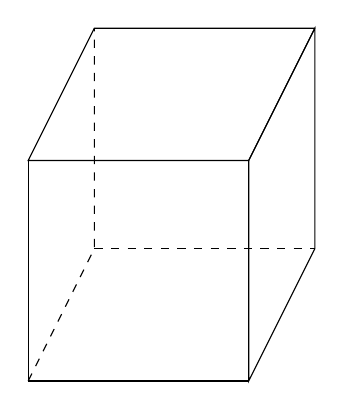
\begin{tikzpicture}[scale=0.28]
	\draw (0,0) -- (10,0) -- (10,10) -- (0, 10) -- cycle;
	\draw (10,0) -- (13,6) -- (13,16) --(10,10) -- cycle;
	\draw (0,10) -- (10,10) -- (13,16) -- (3,16) -- cycle;
	\draw (0,0)[dashed] -- (3,6) -- (3,16);
	\draw (3,6)[dashed] -- (13,6);
	\end{tikzpicture}
\end{minipage}

The file \verb|cube_3.aut| contains the following:
\begin{Verbatim}
Euclidean automorphism group of order 48
Integrality not known
************************************************************************
3 permutations of 8 vertices of polyhedron

Perm 1: 1 3 2 4 5 7 6 8
Perm 2: 1 2 5 6 3 4 7 8
Perm 3: 2 1 4 3 6 5 8 7

Cycle decompositions 

Perm 1: (2 3) (6 7) --
Perm 2: (3 5) (4 6) --
Perm 3: (1 2) (3 4) (5 6) (7 8) --

1 orbits of vertices of polyhedron

Orbit 1 , length 8:  1 2 3 4 5 6 7 8

************************************************************************
3 permutations of 6 support hyperplanes

Perm 1: 1 3 2 5 4 6
Perm 2: 2 1 3 4 6 5
Perm 3: 1 2 4 3 5 6

Cycle decompositions 

Perm 1: (2 3) (4 5) --
Perm 2: (1 2) (5 6) --
Perm 3: (3 4) --

1 orbits of support hyperplanes

Orbit 1 , length 6:  1 2 3 4 5 6
\end{Verbatim}

The automorphism group has order $48$. The system of generators computed by nauty has $3$ elements, listed as permutations of the extreme rays, and, in the second part, as permutations of the facets. \verb|Perm 1: 1 3 2 4 5 7 6 8| says that the first permutation maps vertex $1$ to itself, vertex $2$ to vertex $3$ etc. The reference order of the vertices is the one in which they are listed in \verb|cube_3.out|:
\begin{Verbatim}
8 vertices of polyhedron:
0 0 0 1
0 0 1 1
0 1 0 1
0 1 1 1
1 0 0 1
1 0 1 1
1 1 0 1
1 1 1 1
\end{Verbatim}
The cycle decompositions show that all generators of the euclidean automorphism group have order $2$. It is a good exercise to identify them geometrically.

Both the vertices and the facets form a single orbit for the $3$-cube. As a simple example for which this not the case we take \verb|pythagoras.in|:

\begin{minipage}[b]{0.5\textwidth}
\begin{Verbatim}
amb_space 2
vertices 4
5 0 1
-5 0 1
3 4 1
-3 -4 1
EuclideanAutomorphisms
\end{Verbatim}
\end{minipage}
\hspace{1cm}
\begin{minipage}[t]{0.4\textwidth}
	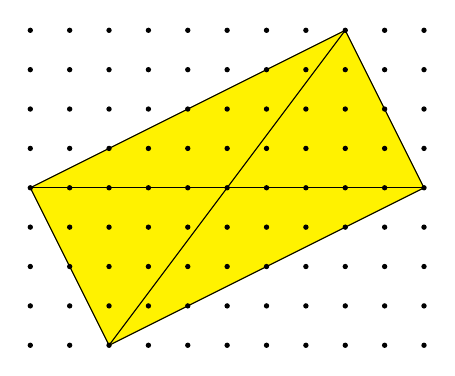
\begin{tikzpicture}[scale=0.5]
	\filldraw[yellow] (5,0) -- (3,4) -- (-5,0) -- (-3,-4) -- cycle;
	\draw (5,0) -- (3,4) -- (-5,0) -- (-3,-4) -- cycle;
	\foreach \x in {-5,...,5}
	\foreach \y in {-4,...,4}
	{
		\filldraw[fill=black] (\x,\y) circle (1.5pt);
	}
	\draw (5,0) -- (-5,0);
	\draw (3,4) -- (-3,-4);
	\end{tikzpicture}
\end{minipage}

We get
\begin{Verbatim}
Euclidean automorphism group of order 4
...
...
2 permutations of 4 support hyperplanes

Perm 1: 2 1 4 3
Perm 2: 1 3 2 4

Cycle decompositions 

Perm 1: (1 2) (3 4) --
Perm 2: (2 3) --

1 orbits of support hyperplanes

Orbit 1 , length 4:  1 2 3 4
\end{Verbatim}
Clearly, this rectangle is not a square.

The euclidean automorphism group of a rational polyhedron with vertices, and in particular the euclidean automorphism group of a pointed cone, is finite and can be computed. For the cone it would be necessary to find points on the extreme rays that have distance $1$ from the origin. In general this requires the extension of $\QQ$ by square roots. In principle such extensions are accessible to Normaliz (see Section~\ref{Algebraic}).

The euclidean automorphisms can only be computed if the input defines a polytope -- it is not enough that the quotient by the maximal subspace does this.


\subsubsection{Rational automorphisms}

Also the computation of rational automorphism groups is restricted to polytopes in Normaliz. Let us take up the rectangle from \verb|pythagoras.in| again, this time asking for rational automorphisms (\verb|pythagoras_rat.in|):
\begin{Verbatim}
amb_space 2
...
RationalAutomorphisms
\end{Verbatim}

Result:
\begin{Verbatim}
Rational automorphism group of order 8
Automorphisms are not integral
************************************************************************
2 permutations of 4 vertices of polyhedron

Perm 1: 1 3 2 4
Perm 2: 2 1 4 3
\end{Verbatim}
This is (hopefully) expected: as an object of rational linear geometry, every rectangle is isomorphic to a square whose automorphism group (in any reasonable sense) is of order $8$, namely the dihedral group of this order.

\subsubsection{Integral automorphisms}

In general, euclidean and rational automorphisms do not map lattice points in polyhedra to lattice points. If we want to exploit automorphism groups in the computation of lattice points or enumerative invariants of polyhedra, we can only depend on integral automorphisms.

Consider a rational pointed cone $C\subset\RR^d$. Let $L\subset\ZZ^d$ be a sublattice such that $L\cap \QQ C$ spans $\QQ C$ (the situation in which we compute Hilbert bases and Hilbert series). We define $\Aut_L(C)$ as the group of rational automorphisms of $C$ that map $L$ onto itself. On the one hand, such an automorphism must permute the Hilbert basis $H$ of the monoid $C\cap L$. On the other hand, $H$ generates the lattice $L$ as a group, and therefore $\Aut_L(C)=\Aut_\QQ(C;H)$. It follows that $\Aut_L(C)$ is a finite group, and that it can be computed as the group of rational automorphisms permuting a finite set of generators of $C$.

For a rational polyhedron $P$ we pass to the cone $C(P)$ and the corresponding extension $L'$ of $L$. Then $\Aut_L(P)$ is the subgroup of $\Aut_{L'}(C(P))$ of those automorphisms that map $P$ onto itself. We simply speak of \emph{integral} automorphisms, assuming that the lattice $L$ is fixed.

If we had to always find the Hilbert basis first, then it would often be very hard to compute integral automorphism groups, and it would be impossible in the future to use the integral automorphisms in the computation of Hilbert bases. Fortunately one often gets away without computing the Hilbert basis, and Normaliz only uses it as the last resort (as in the example below).

Again, let us consider our rectangle, but this time we compute the integral automorphisms (\verb|pythagoras_int.in|).
\begin{Verbatim}
amb_space 2
...
Automorphisms
\end{Verbatim}
Note that integral automorphisms are asked for by \verb|Automorphisms| without an attribute since integral automorphisms are considered the standard choice for Normaliz.

Since an automorphism of a rectangle must permute the diagonals, and these have different numbers of lattice points, the integral automorphisms must fix them, and only the point reflection at the origin remains:
\begin{Verbatim}
Integral automorphism group of order 2
Automorphisms are integral
************************************************************************
1 permutations of 4 vertices of polyhedron

Perm 1: 4 3 2 1
...
\end{Verbatim}

Note that integral automorphisms in general depend on the choice of the reference lattice $L$. For our rectangle $R$, if we replace the full lattice $\ZZ^2$ by the sublattice $L$ spanned by the vertices, then $\Aut_L(R)$ is simply the rational automorphism group of the polytope. You can test this by adding
\begin{Verbatim}
lattice 4
5 0
-5 0
3 4
-3 -4
\end{Verbatim}
to the input file.

\subsubsection{Combinatorial automorphisms}

For polytopes the combinatorial automorphisms are those permutations of the vertices that induce an automorphism of the face lattice. For this property It is necessary and sufficient that they map facets to facets.

As an example we consider the input file \verb|pentagon.in|:

\begin{minipage}[b]{0.5\textwidth}
\begin{Verbatim}
amb_space 2
vertices 5
0 0
1 0
1 1
0.5 1.5
0 1
CombinatorialAutomorphisms
\end{Verbatim}
\end{minipage}
\hspace{1cm}
\begin{minipage}[t]{0.4\textwidth}
	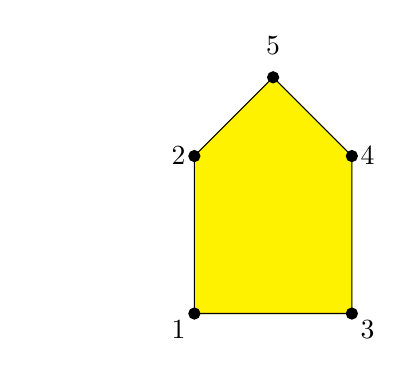
\begin{tikzpicture}[scale=2]
	\filldraw[yellow] (0,0) -- (1,0) -- (1,1) -- (0.5,1.5) -- (0,1) -- cycle;
	\draw (0,0) -- (1,0) -- (1,1) -- (0.5,1.5) -- (0,1) -- cycle;
	\filldraw[fill=black] (0,0) circle (1.0pt);
	\filldraw[fill=black] (1,0) circle (1.0pt);
	\filldraw[fill=black] (1,1) circle (1.0pt);
	\filldraw[fill=black] (0.5,1.5) circle (1.0pt);
	\filldraw[fill=black] (0,1) circle (1.0pt);
	\draw node at (-0.1,-0.1){1};
	\draw node at (-0.1,1.0){2};
	\draw node at (1.1,-0.1){3};
	\draw node at (1.1,1.0){4};
	\draw node at (0.5,1.7){5};
	\draw node at (-1,-0.1){\vphantom{.}};
	\end{tikzpicture}
\end{minipage}

This is a polygon with $5$ vertices. Result (shortened):
\begin{Verbatim}
combinatorial automorphism group of order 10
Integrality not known
************************************************************************
2 permutations of 5 vertices of polyhedron

Perm 1: 1 3 2 5 4
Perm 2: 2 1 5 4 3

Cycle decompositions 

Perm 1: (2 3) (4 5) --
Perm 2: (1 2) (3 5) --

1 orbits of vertices of polyhedron

Orbit 1 , length 5:  1 2 3 4 5
...
\end{Verbatim}


Clearly, every combinatorial automorphism is determined by the values of the two vertices of an edge, and we can freely choose the vertices of any of the five edges as values. So the combinatorial automorphisms group has order $10$, and is in fact the dihedral group of this order. (All other automorphism groups of this pentagon have order $2$.)

\subsubsection{Ambient automorphisms}

Roughly speaking, the ambient automorphisms are those permutations of the coordinates of the ambient space that permute the input vectors. They rae always defined for generator input and for input of inequalities (without an restriction of the lattice or subspace). These automorphisms are always integral and euclidean, but very often they are only a very small subgroup of the group of all integral/algebraic or euclidean automorphisms . The option for them is
\begin{itemize}
	\itemtt[AmbientAutomorphisms]
\end{itemize}
As an example let us take the linear order polytope for $S_6$. If we run
\begin{Verbatim}
./normaliz -c  example/lo6 -i --AmbientAutomorphisms
\end{Verbatim}
then the files \verb|lo6.aut| starts with 
\begin{Verbatim}
Ambient(from generators) automorphism group of order 2 (possibly only approximation)
Automorphisms are integral
************************************************************************
1 permutations of 720 input generators
...
\end{Verbatim}
The linear order polytope  has $10080$ integral automorphisms.

Note that permutations and orbits cannot be computed for factes if the input is by generators or for extreme rays if it is by inequalities since they are simply not known. However, Normaliz prints these data for the coordinates. In the cae  of \verb|lo6|
\begin{Verbatim}
************************************************************************
1 permutations of 16 Coordinates

Perm 1: 15 14 12 9 5 13 11 8 4 10 7 3 6 2 1 16

Cycle decompositions 

Perm 1: (1 15) (2 14) (3 12) (4 9) (6 13) (7 11) --

10 orbits of Coordinates

Orbit 1 , length 2:  1 15
...
Orbit 10 , length 1:  16
\end{Verbatim}
Since the input vectors  are not necessarily printed verbatim in the output file, they appear at the end of the \verb|aut| file:
\begin{Verbatim}
input generators

 1:  1 0 0 0 0 0 0 0 0 0 0 0 0 0 0 0 1 0 0 0 0 0 0 0 0 0 0 0 1 0 0 0 0 0 0 0 0 0 0 0
 2:  0 1 0 0 0 0 0 0 0 0 0 0 0 0 0 0 0 1 0 0 0 0 0 0 0 0 0 0 1 0 0 0 0 0 0 0 0 0 0 0
...
\end{Verbatim}

\subsubsection{Automorphisms from input}\label{input_auto}

For the computation of the input automorphisms Notrmaliz applies the initial coordinate transformations to the input vectors and then computes  their permutations that are given by rational (or algebraic) maps. The option is
\begin{itemize}
	\itemtt[InputAutomorphisms]
\end{itemize}
With
\begin{Verbatim}
./normaliz -c  example/lo6 -i --InputAutomorphisms
\end{Verbatim}
we get indeed the full automorphism group. The permutations of the facets are not computed:
\begin{Verbatim}
Input(from generators) automorphism group of order 10080 (possibly only approximation)
Automorphisms are integral
************************************************************************
3 permutations of 720 input generators
...
\end{Verbatim}
as you can check in the \verb|aut| file. As for ambient automorphisms the input vectors are listed at the end.

\textbf{Note:}\enspace After the initial coordinate transformations, Normaliz reaches
\begin{arab}
\item a full-dimensional primal cone if the input is by generators, or
\item a full-dimensional dual cone if the input is by inequalities,
\end{arab}
but not more. The passage to the full-dimensional pointed primal (or dual) cone is not possible at this point. Therefore the automorphisms computed from raw input do in general not map bijectively to automorphisms of the pointed full-dimensional quotient (or subcone).

Furthermore, in the inhomogeneous case it must be taken into account that Normaliz considers the inequality that makes the homogenizing variable nonnegative as part of the input. This is sometimes necessary to reach a full-dimensional dual cone after the initial coordinate transformation. 

What has just been said is illustrated by \verb|halfspace3inhom-input.in|:
\begin{Verbatim}
amb_space 3
inhom_inequalities 3
1 0 0 1
0 0 1 0
0 0 -1 0
InputAutomorphisms
\end{Verbatim}
We expect an automorphism exchanging the second and the third inequality, and we get it:
\begin{Verbatim}
Input(from inequalities) automorphism group of order 2 (possibly only approximation)
Integrality not known
************************************************************************
1 permutations of 3 input inequalities

Perm 1: 1 3 2

Cycle decompositions 

Perm 1: (2 3) --

2 orbits of input inequalities

Orbit 1 , length 1:  1
Orbit 2 , length 2:  2 3

************************************************************************
input inequalities

1:  1 0  0 1
2:  0 0  1 0
3:  0 0 -1 0
\end{Verbatim}

Compute the \verb|Automorphisms| for this example!

\subsubsection{Monoid automorphisms}\label{mon_auto}

With the computation goal \verb|Automorphisms| Normaliz computes the automorphisms group of an affine  monoisd. These the bijective additive maps from the monoid to itself, and are represen5ted by permutations of the Hilbert basis. An example (\verb|monoid_auto.in|)
\begin{Verbatim}
amb_space 2
monoid 4
2 0
1 1
0 2
0 2
grading
1 1
Automorphisms
\end{Verbatim}
The doubling of the last generator is non-intrinsic for the monoid structure and for the computation of the automorphism group we need intrinsic data:
\begin{Verbatim}
3 Hilbert basis elements:
0 2
1 1
2 0
\end{Verbatim}
The automorphism group is
\begin{Verbatim}
Monoid automorphism group of order 2 (possibly approximation if very large)
Automorphisms are integral
************************************************************************
1 permutations of 3 Hilbert basis elements

Perm 1: 3 2 1

Cycle decompositions 

Perm 1: (1 3) --

2 orbits of Hilbert basis elements

Orbit 1 , length 2:  1 3
Orbit 2 , length 1:  2

************************************************************************
Hilbert basis elements

1:  0 2
2:  1 1
3:  2 0
\end{Verbatim}

Try \verb|InputAutomorphism| and \verb|AmbientAutomorphism| for the same input.

\subsection{Precomputed data}\label{precomputed_data}

The input of precomputed data can be useful if their computation takes long and they can be used again in subsequent computations. Normaliz takes their correctness for granted since there is no way of checking it without recomputation. Nevertheless some consistency checks are done.

We see the main use of precomputed data in interactive access when data had been stored from previous runs and can be made available again. These data allow the reconstruction of a cone (and lattice) and its subsequent modification via \verb|modifyCone| without starting from scratch in the convex hull computation or vertex enumeration.

A file for future input of precomputed data can be asked for by the cone property \verb|WritePreComp|. See Section \ref{write_precomp}.

\subsubsection{Precomputed cones and coordinate transformations}

Precomputed input of this type is given by the homogeneous input types \verb|extreme_rays| and \verb|support_hyperplanes|. (There is a third type \verb|hilbert_basis_rec_cone|; see Section~\ref{HB_rec_cone}.) They can only be used \emph{together}. Moreover, only the following types are allowed with them:
\begin{center}
	\verb|grading, dehomogenization, generated_lattice, maximal_subspace|
\end{center}
This implies that data from inhomogeneous computations must be homogenized and then dehomogenized with explicit \verb|dehomogenization| (see Section~\ref{inhom_prec}). For algebraic polyhedra \verb|generated_lattice| represents a subspace without lattice structure.

Note that support hyperplanes and/or extreme rays do in general not define the object that Normaliz computes: the final pointed object of the computation lives in a subquotient $U/W$ where $U$ is a subspace (or sublattice) of the ambient space $V$ and $W$ is a subspace of $U$. Internally, this information is contained in two coordinate transformations. It is restored via
\begin{arab}
	\item \verb|generated_lattice| for $U$ if $U\neq V$,
	\item \verb|maximal_subspace| for $W$ if $W\neq 0$.
\end{arab}

As an example we consider the input file \verb|tame.in| which has transparent arithmetic:
\begin{Verbatim}
amb_space 4
cone 1
1 0 0 0
subspace 1
0 1 0 0
congruences 1
1 0 0 0 2
\end{Verbatim}
In the output file \verb|tame.out| we find
\begin{Verbatim}
1 extreme rays:
2 0 0 0

1 basis elements of maximal subspace:
0 1 0 0

1 support hyperplanes:
1 0 0 0

...

2 basis elements of generated  lattice:
2 0 0 0
0 1 0 0
\end{Verbatim}
This information is transferred to \verb|tame_prec.in| as
\begin{Verbatim}
amb_space 4
extreme_rays 1
2 0 0 0
maximal_subspace 1
0 1 0 0
support_hyperplanes 1
1 0 0 0
generated_lattice 2
2 0 0 0
0 1 0 0
\end{Verbatim}
Running it reproduces the same output.

\subsubsection{An inhomogeneous example}\label{inhom_prec}
We use the input file \verb|InhomIneq.in| already discussed in Section~\ref{inhom_ineq_ex}:
\begin{Verbatim}
amb_space 2
constraints 3
0 1 >= -1/2
0 1 <=  3/2
-1 1 <=  3/2
grading
unit_vector 1
\end{Verbatim}
In the output file we find
\begin{Verbatim}
dehomogenization:
0 0 1 

grading:
1 0 0 

...

2 vertices of polyhedron:
-4 -1 2
0  3 2

1 extreme rays of recession cone:
1 0 0

3 support hyperplanes of polyhedron (homogenized):
0 -2 3
0  2 1
2 -2 3
\end{Verbatim}
The coordinate transformations are trivial in this case. The translation into an input file with precomputed data is \verb|InhomIneq_prec.in|:
\begin{Verbatim}
amb_space 3
extreme_rays 3
-4 -1 2
0  3 2
1  0 0
support_hyperplanes 3
0 -2 3
0  2 1
2 -2 3
grading
1 0 0
dehomogenization
0 0 1
\end{Verbatim}
The vectors from the output can be copied. But there are two points to note:
\begin{arab}
	\item The change of \verb|amb_space| from~$2$ to~$3$.
	\item The \verb|extreme_rays| unite the vertices of the polyhedron and the extreme rays of the recession cone.
\end{arab}


\subsubsection{Precomputed Hilbert basis of the recession cone}\label{HB_rec_cone}

In applications one may want to compute several polyhedra with the same recession cone. In these cases it is useful to add the Hilbert basis of the recession cone to the input. An example is \verb|small_inhom_hbrc.in|:
\begin{Verbatim}
amb_space 6
cone 190
6 0 7 0 10 1
...
vertices 4
0 0 0 0 0 0 1
1 2 3 4 5 6 2
-1 3 9 8 7 1 3
0 2 4 5 8 10 7
hilbert_basis_rec_cone 34591
0  0  0  1  6 1 0
0  0  0  1  7 1 0
...
\end{Verbatim}
As in the other cases with precomputed data, Normaliz must believe you and the precomputed Hilbert basis of the recession cone does not define the latter.

It requires inhomogeneous input. Note that it can only be used in the primal algorithm. In the dual algorithm it is useless and therefore ignored.

\subsection{Singular locus}\label{SingularLocus}

Certain data of affine monoid algebras are accedssuble by purely combinatorial methods. In particular this is true for the singular locus. (See SEction \ref{local_prop}.) It is computed by
\begin{itemize}
	\itemtt[SingularLocus]
\end{itemize}
For \verb|monoid.in| (see Section \ref{moninp_def}) the output file contains
\begin{Verbatim}
codim singular locus = 1
\end{Verbatim}
and the file with suffix
\begin{itemize}
	\itemtt[sng] contains the singular locus.
\end{itemize}
The format is the same as that for the face lattice:
\begin{Verbatim}
2
5

00010 1
00001 1
\end{Verbatim}
The last integer in each row is the codimension of a minimal singular prime ideal and the face opposite to it is the intersection of the support hyperplanes with entry $1$ in the $0$-$1$-vector. The codimension $1$ is not surprising for a nonnormal monoid.

If we are only interested in the codimenasion, we ask for
\begin{itemize}
	\itemtt[CodimSingularLocus] computing the codimension of the singular locus
\end{itemize}
or only
\begin{itemize}
	\itemtt[IsSerreR1] checking the Serre property $(R_1)$
\end{itemize}
which means that the codimension of the singular locus is $\ge 2$. If this is all you want to know, then use \verb|IsSerreR1| since it avoids the computation of the face lattice.

\subsection{Packed format in the output of binomials}\label{BinomialsPacked}

Output files of binomials are often very sparse, i.e., contain many entries $0$. Reading them by computer  algebra systems with a file interface like Singular or Macaulay2 can therefore be time consuming. To speed reading up, we have introduced a packed format for binomial output files.
\begin{itemize}
	\itemtt[BinomialsPacked] activates the packed format for binimial output files.
\end{itemize}
For \verb|representations.in| (discussed in Swction \ref{markov}) it turns \verb|representations.rep| into
\begin{Verbatim}
-4
8
4 1 -1 3 -1 4 -1 5 1 
3 3 -1 4 -2 6 1 
4 1 -1 3 -2 4 -3 8 1 
4 1 -2 2 1 3 -3 4 -2
\end{Verbatim}
The negative entry in the first line indicates the packed format. Its absolute value is the number of rows. Each row starts with the number vof nonzero entries, and each such entry is given by a pair (column, value).



